% !TeX program = xelatex
% =============================================================================
%  2026 全国大学生嵌入式芯片与系统设计竞赛 · AMD 赛道 3.3 自主选题
%  技术文档（严格按官方《技术文档模板》五部分结构）
%  编译：xelatex report-1031.tex  跑两遍（第二遍生成目录/交叉引用）
%  依赖：TeX Live / MiKTeX + ctex（中文字体用 Windows 自带宋体/黑体）
%
%  占位符（提交前全文搜索“待填/此处插图”清空）：
%    \TODO{...}    红色小字 = 必须由人填的客观事实（编号、组别、型号、心得）
%    \NEEDFIG{...} 红色方框 = 此处应插入的图，框内写明“插什么图、为什么、怎么拍”
%  说明：模板页眉的 logo 已从 技术文档模板.docx 的 word/media/image1.png 提取为
%        template-logo.png，由 fancyhdr 每页显示；正文 5 幅图为 TikZ 原地绘制。
% =============================================================================
\documentclass[UTF8,a4paper,zihao=5,fontset=windows]{ctexart}

\usepackage[a4paper,left=3.17cm,right=3.17cm,top=2.54cm,bottom=2.54cm,
            headsep=0.45cm,footskip=0.9cm]{geometry}
\usepackage{xcolor}
\usepackage{graphicx}
\usepackage{booktabs}
\usepackage{tabularx}
\usepackage{array}
\usepackage{longtable}
\usepackage{multirow}
\usepackage{enumitem}
\usepackage{caption}
\usepackage{float}
\usepackage{fancyhdr}
\usepackage{amsmath}
\usepackage{listings}
\usepackage{tikz}
\usetikzlibrary{arrows.meta,positioning,fit,backgrounds,calc}
\usepackage[hidelinks]{hyperref}

% ---------- 颜色 ----------
\definecolor{todoc}{RGB}{200,30,30}
\definecolor{tbdc}{RGB}{185,100,0}
\definecolor{tbdbg}{RGB}{255,246,232}
\definecolor{photoc}{RGB}{120,120,120}
\definecolor{photobg}{RGB}{246,246,246}
\definecolor{bluec}{RGB}{30,70,140}

\captionsetup{font=small,labelsep=quad}
\setlist{nosep,leftmargin=2.2em}
\setlength{\emergencystretch}{3em}
\renewcommand{\arraystretch}{1.15}

% ---------- 三类占位符 ----------
\newcommand{\TODO}[1]{{\color{todoc}\textbf{[待填：#1]}}}
\newcommand{\TBD}[1]{%
  \begin{center}\setlength{\fboxsep}{6pt}%
  \colorbox{tbdbg}{\parbox{0.94\linewidth}{\color{tbdc}\small\textbf{[静态/动态 二选一]}\ #1}}%
  \end{center}}
\newcommand{\PHOTO}[1]{%
  \begin{center}\setlength{\fboxsep}{12pt}%
  \fcolorbox{photoc}{photobg}{\parbox[c][2.3cm][c]{0.86\linewidth}{\centering\color{photoc}\small #1}}%
  \end{center}}
\newcommand{\code}[1]{\texttt{\small #1}}
\newcommand{\figph}[1]{\PHOTO{#1}}

% \NEEDFIG：红字 + 红框，说明"此处需要插入一张什么样的图"
\definecolor{needc}{RGB}{199,32,32}
\newcommand{\NEEDFIG}[1]{%
  \begin{center}\setlength{\fboxsep}{7pt}%
  \fcolorbox{needc}{white}{\parbox{0.9\linewidth}{\color{needc}\small
    \textbf{[此处插图]}\ #1}}%
  \end{center}}

% -----------------------------------------------------------------------------
% 缺图软失败补丁（2026-10-31）
% 队友新增的 images/*.png|jpg 若未随 tex 一起拷入 docs/images/，\includegraphics 会
% 直接报错并中断编译，产出被截断的 PDF。此处把 \includegraphics 包一层：文件存在则正常
% 插入，不存在则画一个红色提示框并继续编译。图片拷齐后**无需改动任何 \includegraphics**。
% -----------------------------------------------------------------------------
\makeatletter
\let\rtcs@includegraphics\includegraphics
\newcommand{\MISSINGFIG}[1]{%
  \setlength{\fboxsep}{8pt}%
  \fcolorbox{needc}{white}{\parbox[c][2.6cm][c]{0.86\linewidth}{\centering
    \color{needc}\small\textbf{[缺图片文件]}\\[3pt]
    \texttt{#1}\\[3pt]
    把 \texttt{images/} 目录整份复制到 \texttt{docs/} 下，此图会自动出现}}}
% 图片实际落在 Zynq-6DOF-RTCS/images/ 下（tex 与其同级），故先按原路径找，
% 找不到再补 Zynq-6DOF-RTCS/ 前缀；两处都没有才画缺图框。
\newcommand{\rtcs@imageroot}{Zynq-6DOF-RTCS/}
\renewcommand{\includegraphics}[2][]{%
  \IfFileExists{#2}{\rtcs@includegraphics[#1]{#2}}{%
    \IfFileExists{\rtcs@imageroot#2}{\rtcs@includegraphics[#1]{\rtcs@imageroot#2}}{%
      \MISSINGFIG{#2}}}}
\makeatother

\lstset{basicstyle=\ttfamily\scriptsize,breaklines=true,frame=single,
        columns=fullflexible,keepspaces=true,showstringspaces=false}

% 章节号：一级显示“第一部分”，二级仍用 1.1 形式（与官方模板一致）
\renewcommand{\thesection}{第\chinese{section}部分}
\renewcommand{\thesubsection}{\arabic{section}.\arabic{subsection}}
\renewcommand{\thesubsubsection}{\arabic{section}.\arabic{subsection}.\arabic{subsubsection}}

% 目录只收三级（章/节/小节）；\paragraph 级的“（一）……”属正文小节内的编号，
% 放进目录会把两页目录撑满且逐条无助于检索，故 tocdepth 设为 3。
\setcounter{tocdepth}{3}

% 页眉：对齐官方模板——logo 居中，下边框 single / 0.75 pt（模板 styles.xml 中 header 样式
% 为 w:bottom val=single sz=6 space=1，sz 以 1/8 pt 为单位即 0.75 pt）
\setlength{\headheight}{1.5cm}
\pagestyle{fancy}
\fancyhf{}
\renewcommand{\headrulewidth}{0.75pt}
\renewcommand{\headrule}{\hbox to\headwidth{\color{black}%
  \leaders\hrule height \headrulewidth\hfill}}
\fancyhead[C]{
\includegraphics[height=1.02cm]{template-logo.png}}
\fancyfoot[C]{\small \thepage}

% =============================================================================
\begin{document}

% ------------------------- 第 1 页：作品名称 + 团队信息 + 摘要 -----------------
% 版式要求：作品名称/团队信息与摘要同处一页，目录独占第 2 页，正文从第 3 页起。
\begin{center}
  {\zihao{2}\bfseries Zynq 六轴机械臂视觉引导抓取系统}\\[5pt]
  {\large ——面向流水线异常品剔除的视觉分拣与六轴实时执行}\\[9pt]
  {\small 参赛编号：49824\quad 参赛赛道：AMD 自主选题\quad
   组别：初级组}\\[2pt]
  {\small 2026 年 10 月 31 日}
\end{center}

\vspace{-2pt}
\section*{\texorpdfstring{摘\quad 要}{摘要}}
\addcontentsline{toc}{section}{摘要}

流水线上的异常品剔除的难点集中在低抖动和高精度：带速越快，从相机看到、程序判到机械臂执
行，中间可用的时间越短；异常品密度又随批次起伏，稀疏和密集两种工况很难用同一套节拍
兼顾。常见方案多用单片机主控舵机，视觉再单独成模块，协议转换和调度环节偏多。Zynq 的
PS 和 PL 分工更适合这类任务：PS 端运行 Linux 镜像程序，做舵机状态判断和抓取姿态解算；PL 端直接
连六轴舵机，按硬件时序下发运动指令，可以实现更低的抖动和更高的精度。本作品是一套六轴机械臂视觉
分拣系统，按异常品密度切换连续抓取和批次拣选两种模式。

图像检测以及抓取点判断放到上位机前端，输出只有一对毫米坐标和一个执行结论；Zynq-7020 的 PL 里
实现六轴舵机总线协议时序、六轴同帧广播、逐轴限位和截止时间检查，PS 只负责坐标到关节的映射和任务
编排。视觉不用深度相机，也不做传统内参标定，带面四点单应把像素直接换成毫米坐标；机械臂上跳过解析
逆解这一系列复杂的链路，用现场对应点把“像素—关节”这一整体过程直接记成分段关系，直接从映射算出关节目标；
误差不再沿内参、位姿和连杆参数逐级传递，既可测又可复现，也省去标定板。

与常见的实现相比，我们的实现差异在以下三处：\textbf{一是相对“单片机主控+独立视觉模块”}，其坐标需要经过多次
协议转换才能到达执行端，在这里视觉和运动控制都在一块 Zynq 上，坐标通过串行链路直达PL，总线换向和组帧
都由硬件来完成，不经过操作系统的调度，所以控制周期更稳；\textbf{二是相对“手眼标定+解析逆运动学”}，
误差会沿相机内参、安装位姿、连杆参数逐级传递；在这里我们把“像素到关节”当成一个整体，用带面四点单应加
上六舵机坐标示教插值直接拟合，误差主要看示教重复性，可以测也可以复现，还省掉了标定板；\textbf{三是
相对“分层中间件架构”}，带速一高每次排队抖动就落到落点上，由于本作没有中间层，指令路径更短，误差来源也清楚，
同带速下也不必靠降速补精度。

在 295--420\,mm 行程上带速 60--67\,mm/s 连续运行时，连续抓取各类工件
16 轮成功完成抓取、放置、复位 15 次，完整一轮 8.6\,s；停机批次拣选连续 13 次全部成功。可编程逻辑 LUT 占用 12.7\%，
100\,MHz 时钟下时序收敛。

\vspace{3pt}
\noindent\textbf{关键词}：Zynq-7020；六轴机械臂；视觉分拣；预测拦截；平面单应；实时总线控制

% ---------------------------- 第 2 页：目录 ---------------------------------
% 注意：目录条目来自 .toc，必须连续编译两遍才会出现（第一遍只写出 .toc）。
\newpage
\tableofcontents
\newpage

% =============================================================================
\section{作品概述}

\subsection{功能与特性}

本作品是一套面向流水线的\textbf{异常品分拣单元}。工件分两类，圆柱为合格件，正方体等其他物件为
异常件。系统只把异常件拣出、合格件随带通过；操作者把工件随意放上带面，全程无需输入
坐标。按异常品的分布密度提供两种工作模式。

（1）\textbf{连续抓取}，用在异常件少而分散的时候。传送带连续运行，机械臂在高位待命；视觉在
工件进入触发线后估算带速并预测拦截点，机械臂按预测时刻推进、到位即闭合夹爪。

（2）\textbf{批次拣选}，用在异常件多而集中的时候。输送带先以最高速把整批工件送到工位后停机，
机械臂在静止带面上逐件分拣，按位置依次抓取并避免对同一工件重复触发。

（3）\textbf{类别分流}。视觉输出异常物体与圆柱两类目标，只对异常类下发抓取指令，
合格件不占用节拍。

（4）\textbf{夹持状态自判}。夹爪闭合受阻后读回舵机位置，能区分“夹住工件”与“空夹”，
两者相差 150 个位置单位以上，无需加装力觉或光电传感器。

（5）\textbf{异常不中断作业}。舵机故障分为可屏蔽（夹持时的短时过载）与不可屏蔽
（通讯、限位）两类，前者按轴屏蔽、后者照常上报并安全停机；告警本身不会中止当前任务。

\begin{figure}[H]\centering
\begin{minipage}[t]{0.47\linewidth}\centering
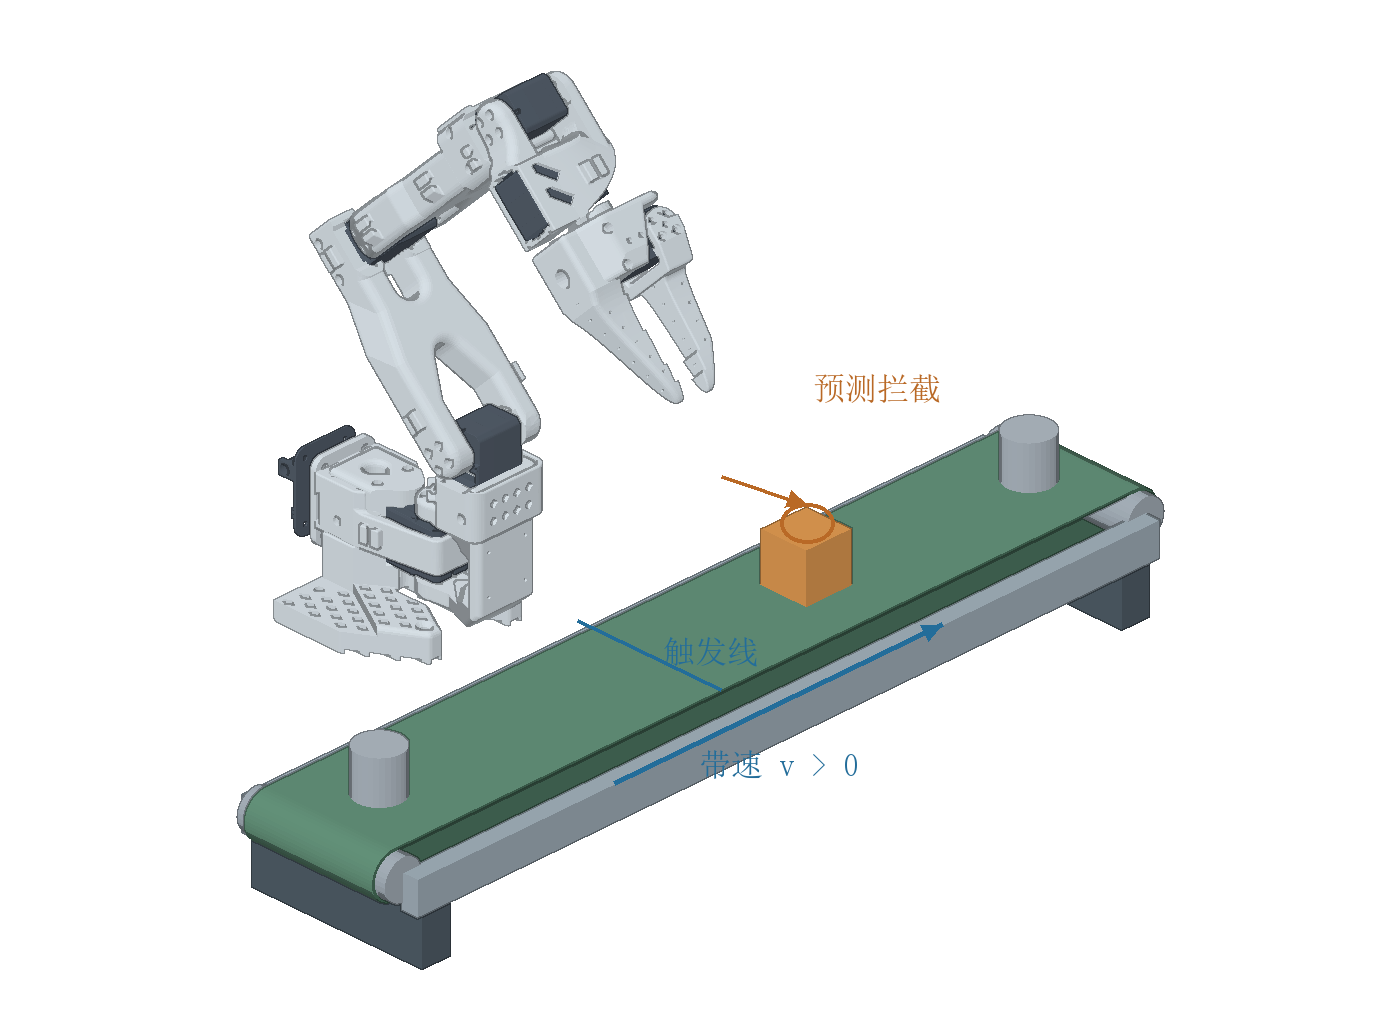
\includegraphics[width=0.92\linewidth]{images/mode-follow-grasp.png}
\par\smallskip{\small （a）连续抓取}
\end{minipage}\hfill
\begin{minipage}[t]{0.47\linewidth}\centering
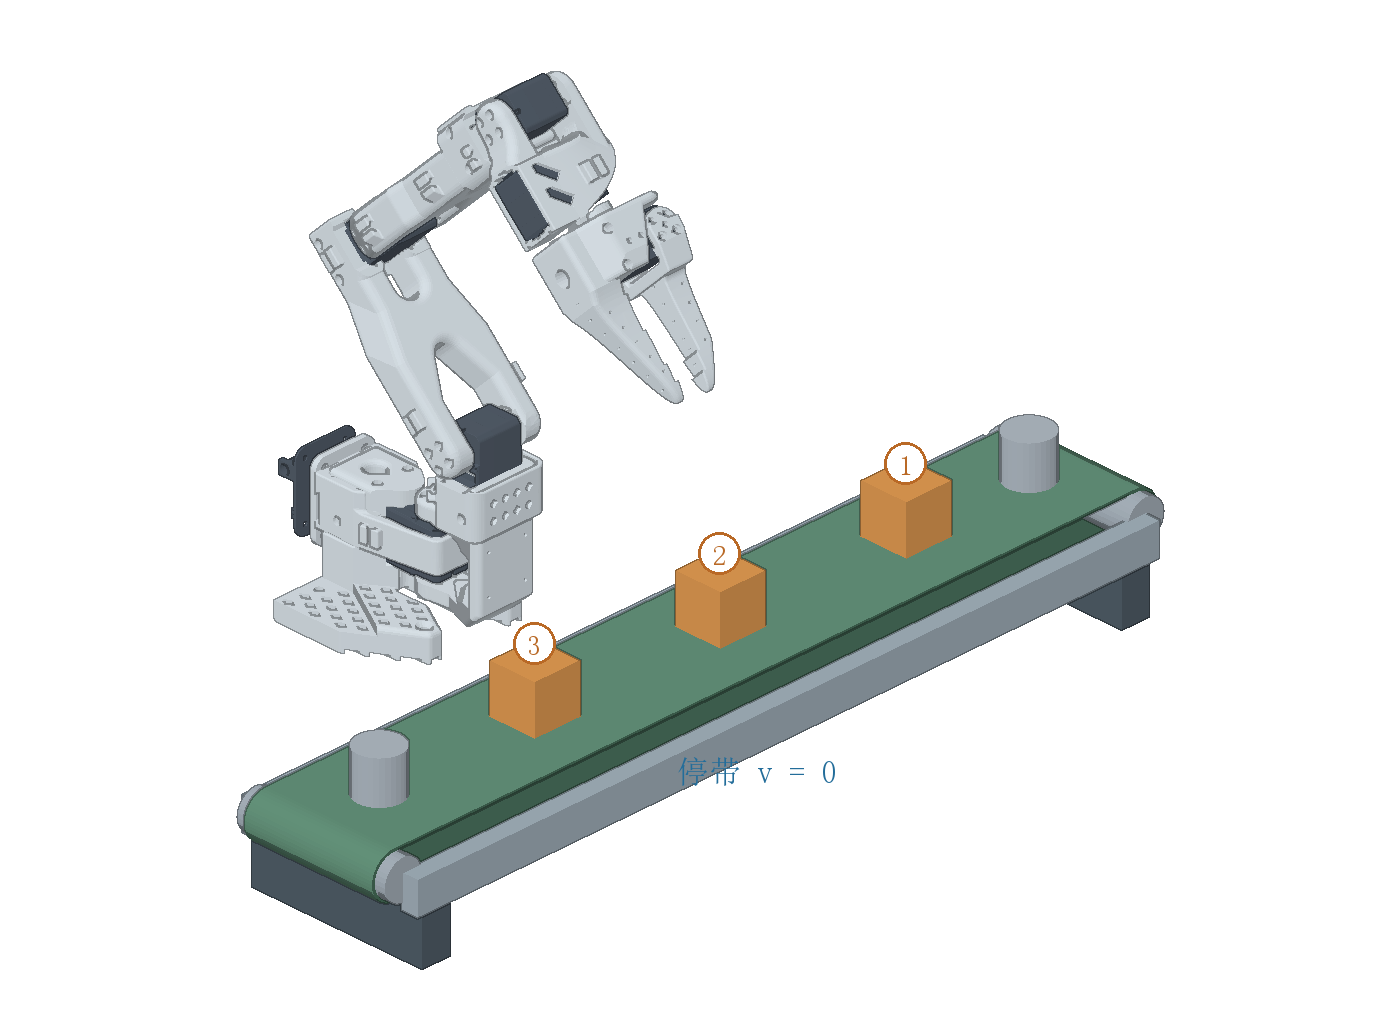
\includegraphics[width=0.92\linewidth]{images/mode-batch-pick.png}
\par\smallskip{\small （b）批次拣选}
\end{minipage}
\par\smallskip
{\footnotesize 方块等为异常件，圆柱为合格件；机构与动作关系为示意。}
\caption{连续抓取与批次拣选两种工作模式}\label{fig:two-operation-modes}
\end{figure}



\subsection{应用领域}

本作品对准产线上的\textbf{来料异常品剔除工位}。以注塑车间为例，一条线连续
生产同款外壳，换模或混料时偶有几只上一款混进来，尺寸相差不大，人工抽检比较困难。当它流到
装配线时会卡住夹具，逼停整条产线，不翻出来就开不了线。如果加装专用剔除机构
的话性价比不高，因为一种机构只解决一种缺陷，换型还得改机械对位。

本作品\textbf{不改产线}，只加一个工位，一根相机横杆加一只六轴臂，串在输送带末端，不接产线
PLC、不取电机信号、不与传送带通信，非常方便。换型只换标定与判定规则，机械结构仍然不变，这是它相对专用
器械最实际的价值。

更实用的一点是\textbf{按密度换策略}。异常品零星出现时不停产线，臂在带面上方跟上去拦截，抓完
即回位；异常品成批出现时把整批料送到工位后停机，逐件确认、逐件拣出，宁可慢也不漏。一套
硬件与视觉，按工况换节拍，不必为两种工况买两套设备。

同一思路可复制到包装线缺件与异物剔除、3C 来料超差分选；也适合做教学平台，演示
“看见—判断—执行”闭环。

\subsection{主要技术特点}

（1）\textbf{平面标定}。作业面本身就是平面，因此不做内参标定，也不用标定板、标定球：
程序用绿色掩膜加最小外接矩形自动找出带面四角，与 490\,mm$\times$80\,mm 的物理尺寸
建立单应矩阵，人工确认一次存成标定文件；畸变、倾角与安装高度一并纳入这一次映射，带面内
不再单独建模。相机或基座挪动后重跑一次即可，标定物一件也不需要。

（2）\textbf{实测舵机坐标示教表}。解析逆运动学需要标定连杆长度、关节零点与
轴间耦合，误差源多且难以单独验证；本方案在带面六个位置逐一读取各关节的实际位置值
（舵机 count），构造分段线性插值，误差上限由示教的重复定位精度决定，可测、可复现。

（3）\textbf{带速每轮重估，拦截点当场解算}。输送带的实际速度会随负载与电压波动，用固定
值会积出可观的提前量误差；系统每轮以最近若干帧的位移做最小二乘拟合得到当前带速，再由
飞行时间反算本轮拦截点，匀速工况下提前量误差落在毫米级。

（4）\textbf{出点前先判稳定}。抓取点由多帧定，取最近一段“$x$、$y$ 极差均不超过
2\,mm”的最长后缀，跨度满 0.5\,s 才有效，坐标取该段中位数；目标静止不足时长或仍在抖动
时就不出点，只把当前极差打进日志。

（5）\textbf{实时任务由可编程逻辑完成}。总线换向、组帧、校验、六轴同帧广播、逐轴限位
与截止时间判定均在可编程逻辑（PL）内按 100\,MHz 时钟完成；处理器系统（PS）只做坐标解算、
七步任务编排与夹持判定，向 PL 下发目标值。上位机到舵机之间只有“一对坐标下行、一个结论
上行”，不经过任何中间件进程。

\subsection{主要性能指标}

静态（模式二）闭环 13/13（覆盖 300--403\,mm），动态（模式一）在 60.4--66.7\,mm/s
下 15/16；定位重复性 $\pm$0.15\,mm，落点偏差 0.1--1.2\,mm；PL 占 LUT 12.69\%、
FF 10.84\%，100\,MHz 时序全满足。详见表~\ref{tab:perf}。

\begin{table}[H]\centering\small
\caption{主要性能指标}
\label{tab:perf}
\begin{tabularx}{\linewidth}{@{}p{3.3cm}p{3.7cm}X@{}}
\toprule
指标 & 数值 & 测量条件 / 备注 \\
\midrule
模式二 静态抓取成功率 & \textbf{13/13} & 40\,mm 方块，$y$ 限 36$\pm$5\,mm，传送带静止 \\
模式一 连续抓取成功率 & \textbf{15/16} = 93.8\% & 带速 60.4--66.7\,mm/s；17 次触发含 1 次未越线 \\
模式二 单轮周期 & P50 \textbf{7.84}\,s & 收到坐标$\rightarrow$exit 到位，含视觉与串口 \\
模式一 完整一轮 & P50 \textbf{8.6}\,s & 视觉出点、抓取搬运、回待命位都在内 \\
可抓取区间 & 295--420\,mm & 六点示教表覆盖；动态拦截点 350\,mm \\
定位重复性 & $\pm$0.15\,mm & 同一物理点三次读数极差 \\
落点偏差 & \textbf{0.1--1.2}\,mm & 预测落点 vs 实际咬合位置 \\
臂到位抖动 & \textbf{4--19}\,ms & 折合 63\,mm/s 下 0.25--1.2\,mm \\
信号发送误差 & 3.5--18.7\,ms & 串口上行时刻误差 \\
夹持判据 & 2364--2409 / 2214--2216 & 夹住堵转位 / 夹空合到底，相差 $>$150 count \\
PL 资源占用 & LUT 12.69\%、FF 10.84\% & XC7Z020，Vivado 2023.2 impl 后 \\
主时钟与时序 & 100\,MHz，全约束满足 & \code{clk\_fpga\_0}，无违约端点 \\
\bottomrule
\end{tabularx}
\end{table}

\subsection{主要创新点}

（1）\textbf{用直连架构换出时间预算}。视觉→坐标→关节→总线帧不跨中间件，落点偏差
0.1--1.2\,mm；按 63\,mm/s 折算，这只等于 2--19\,ms 的时间窗。分层中间件式的机器人栈
（如基于 ROS 的节点图）每层都有序列化与调度排队，十毫秒级的抖动会直接变成毫米级偏差，
因此同等精度下只能降带速；本方案能把线速拉到 60\,mm/s 以上，原因就在这里。

（2）\textbf{按异常件密度切换两种抓取模式}，同一套链路覆盖“稀疏连续抓取”与“密集批量拣选”。

（3）\textbf{夹持状态用堵转位与闭合耗时双判据自动判定}，不加传感器即区分夹住与夹空。

（4）\textbf{故障分级为可屏蔽/不可屏蔽}，既不因过载误停，也不掩盖通讯故障。

\subsection{设计流程}

需求分析（工件尺寸、抓取区间、节拍）$\rightarrow$ 平台选型（Zynq-7020 + 总线舵机）
$\rightarrow$ 驱动器与 PL 逻辑打通 $\rightarrow$ 平面标定与检测链路 $\rightarrow$
七步状态机与示教表 $\rightarrow$ 静态闭环联调 $\rightarrow$ 带速实测与预测拦截
$\rightarrow$ 指标实测与证据归档，见图~\ref{fig:flow}。

\begin{figure}[H]\centering
\begin{tikzpicture}[
  node distance=3.2mm,
  box/.style={draw,rounded corners=2pt,fill=blue!6,align=center,inner sep=3pt,
              font=\scriptsize,minimum height=8mm,text width=20mm},
  ar/.style={-{Latex[length=1.6mm]},draw=bluec,thick}]
\node[box] (a) {需求分析\\尺寸/区间/节拍};
\node[box,right=of a] (b) {平台选型\\Zynq-7020\\总线舵机};
\node[box,right=of b] (c) {PL 逻辑\\协议/限位\\deadline};
\node[box,right=of c] (d) {平面标定\\四点单应\\检测链路};
\node[box,right=of d] (e) {七步状态机\\六点示教表\\夹持判据};
\node[box,below=8mm of d] (f) {闭环联调\\静态→动态\\串口直传坐标};
\node[box,left=of f] (g) {指标实测\\成功率/周期\\精度};
\node[box,left=of g] (h) {证据归档\\日志/录像\\指标表};
\draw[ar] (a)--(b); \draw[ar] (b)--(c); \draw[ar] (c)--(d);
\draw[ar] (d)--(e); \draw[ar] (e.south) |- (f.east);
\draw[ar] (f)--(g); \draw[ar] (g)--(h);
\end{tikzpicture}
\caption{设计流程}
\label{fig:flow}
\end{figure}

% =============================================================================
\section{系统组成及功能说明}

\subsection{整体介绍}

系统由四层构成：\textbf{感知层}（相机 + 上位机视觉程序）、\textbf{决策层}（上位机抓取点
决策与任务下发）、\textbf{编排层}（板端 PS 的坐标$\rightarrow$关节映射与七步状态机）、
\textbf{执行层}（PL 的总线时序逻辑 + 六个总线舵机）。四层的物理边界与数据流见
图~\ref{fig:arch}。

\begin{figure}[H]\centering
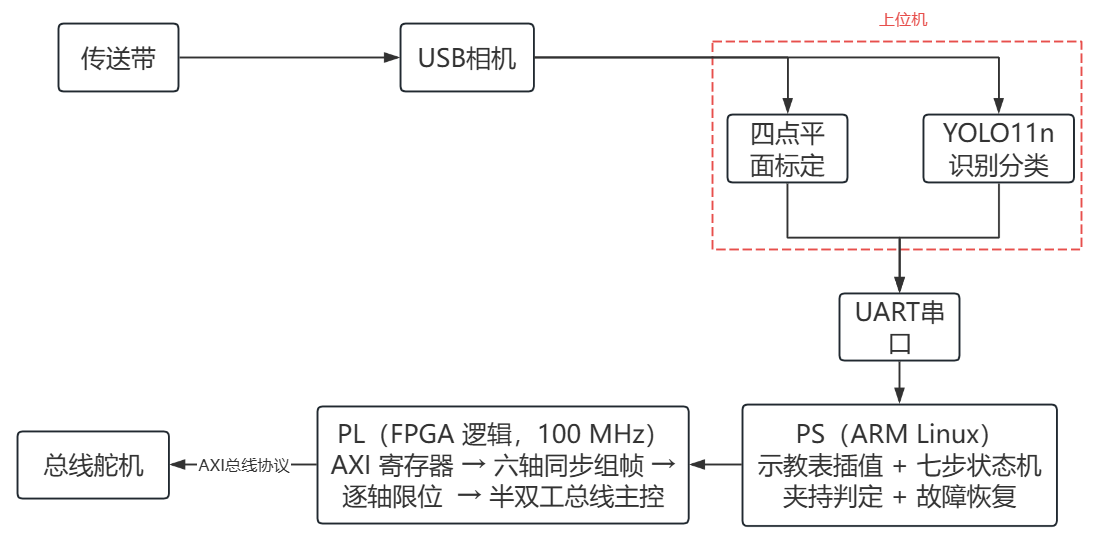
\includegraphics[width=\linewidth]{images/全流程.png}
\caption{系统整体框图：上位机（红框）完成四点标定与 YOLO11n 识别，经 UART 串口下发；
PS 负责示教表插值与七步状态机，PL 负责六轴同步组帧与限位校验，经总线协议驱动总线舵机}
\label{fig:arch}
\end{figure}

各模块之间的关系为：上位机只向板端下发一对
毫米坐标，板端只向上位机回报一次抓取结论（成功/夹空 + 接触位置 + 周期），其余状态全部
在板内闭环。这样设计的理由是：坐标是唯一需要“看”的量，结论是唯一需要“留痕”的量，
其余都跨链路传递时，并不增加信息。

两种模式共用这一条链路，差别只在决策层：模式二（批次拣选）由上位机在传送带静止时
取点、逐件下发，属于“看准了再动”；模式一（连续抓取）由上位机判断“何时该动”，
把预测出的拦截点与触发时刻一起下发。执行层与编排层完全复用，
这也是同一套代码能覆盖两种工况的原因。

\subsection{硬件系统介绍}

\subsubsection{硬件整体介绍}

主控为 ALINX AX7Z020（Xilinx Zynq-7020，XC7Z020），PS 为双核 Cortex-A9 + 1\,GiB DDR3，
PL 为 85K 逻辑单元。板卡通过 AXI4-Lite 寄存器组对外暴露一个版本化的软硬件接口
（ABI \code{0x5254000E}），PS 侧命令行与 PL 逻辑按该 ABI 解耦，便于两侧独立升级。

执行器为 6 个 HX-30HM 总线舵机（ID1--5 为关节，ID6 为夹爪），共用一根半双工信号线。

视觉侧为一个 1280$\times$720 免驱 UVC 相机。
上位机与板卡之间用 USB-UART（115200\,8N1）连接，该链路同时是板卡控制台，
因此软件上做了“一条链路两种用途”的分时复用。

PL 侧资源与时序（Vivado 2023.2，impl 后）：LUT 6\,751（12.69\%）、FF 11\,537
（10.84\%）、BRAM 0、DSP 2（0.91\%），主时钟 \code{clk\_fpga\_0} 100\,MHz，
“All user specified timing constraints are met”。

\subsubsection{机械设计介绍}
\label{sec:mechanical-design}
机械系统由机械臂、末端二指夹爪、输送带、固定相机及基座夹紧组件构成。机械臂沿用 SO-ARM101 类开源套件结构，白色打印件通过舵机、舵盘与紧固件连接；ID1--ID5 调整末端位姿，ID6 独立驱动夹爪开合。本文的“六轴”对应六路舵机执行通道。本作品的机械工作主要为固定工位搭建、安装布置及抓取任务适配。

\noindent\textbf{（1）整机布局与固定安装}

如图~\ref{fig:mechanical-layout-design} 所示，输送带水平布置，机械臂基座安装在带侧，末端夹爪由侧方进入抓取区域；相机独立固定在带面上方。固定相机用于观察工件，不安装在腕部。该布局将输送、观测和执行组织在同一工位内，并为夹爪接近与抬升留出空间。

机械臂采用底板支承及螺杆夹紧组件固定于工作台，舵机线束沿臂段外侧整理，在关节处保留弯曲余量。装配后检查基座紧固、线束牵拉和运动干涉，再在固定工位完成平面标定与关节示教；若相机或基座移动，应重新核对相应标定关系。
\begin{figure}[H]\centering
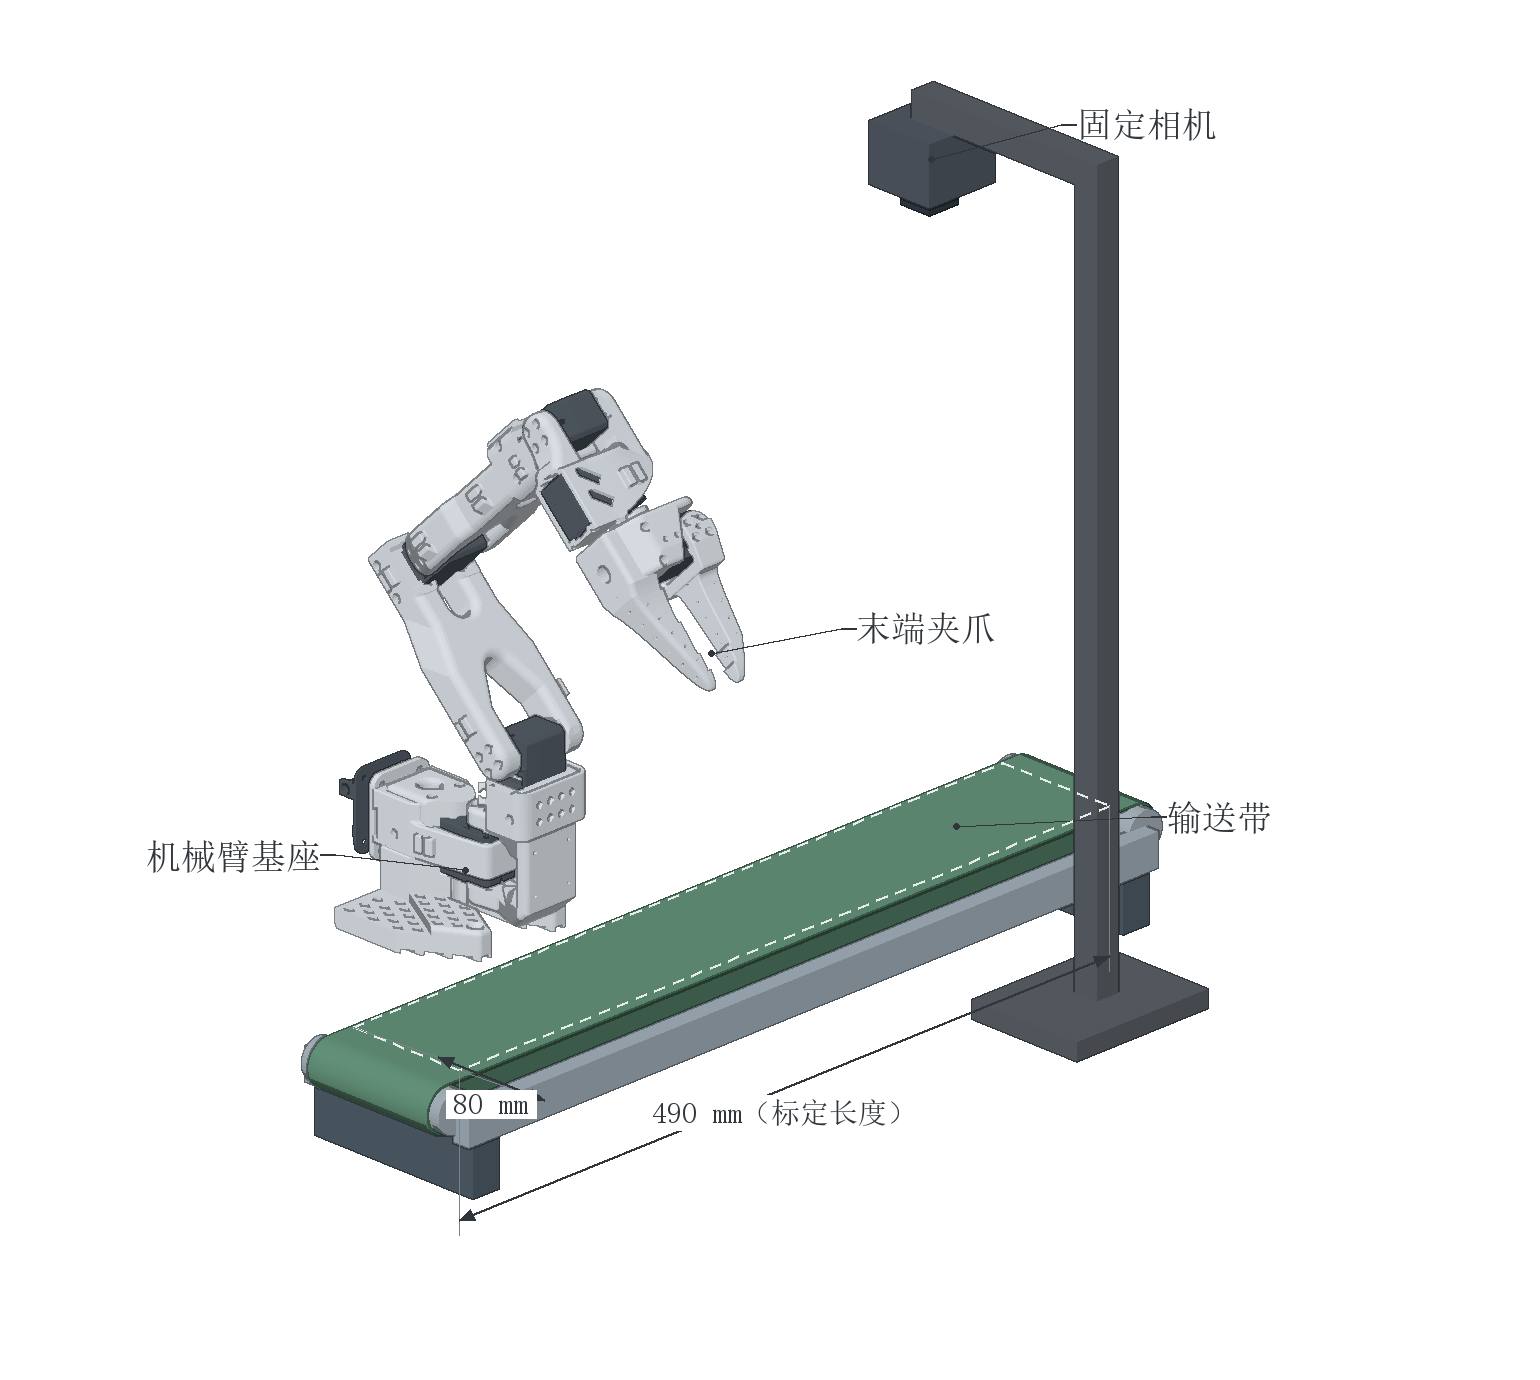
\includegraphics[width=0.98\linewidth]{images/cad-workstation-layout-annotated.png}
\caption{整机布局与带面标定区域}\label{fig:mechanical-layout-design}
\end{figure}

图中机械臂直接取自厂家提供的白色从臂 CAD，隐藏了实物未使用的腕部相机附件；相机及输送带采用简化模型表达安装关系。虚线框内的 490\,mm$\times$80\,mm 为带面标定区域，不是输送带外形尺寸。镜头至带面高度、基座至输送带的安装距离尚待现场确认，图中未按比例给出这些数值；模型姿态也不表示实测抓取姿态。

\noindent\textbf{（2）夹爪与腕部结构及进入余量}

腕部连接姿态调整关节与末端二指夹爪，局部结构如图~\ref{fig:gripper-cad-clearance} 所示。夹爪张开后使方块进入两指之间，闭合夹持后先抬升、再转向放置区。对于边长 40\,mm 的方块，以实际进入深度处的两指内侧净距 $W_{\mathrm{open}}$ 表示有效开口，居中且对正时单侧几何余量为
\[
\Delta=\frac{W_{\mathrm{open}}-40\,\mathrm{mm}}{2}.
\]
依据先前提供的带尺照片（不收入本文），两指内缘沿尺面约对应 10.0\,cm 与 16.5\,cm，照片估读 $W_{\mathrm{open}}\approx65\,\mathrm{mm}$。由此得到总余量约 25\,mm，居中时单侧约 12.5\,mm。下图的尺寸关系示意用于说明工件进入条件，独立于 CAD 文件中保存的夹爪姿态。

\begin{figure}[H]\centering
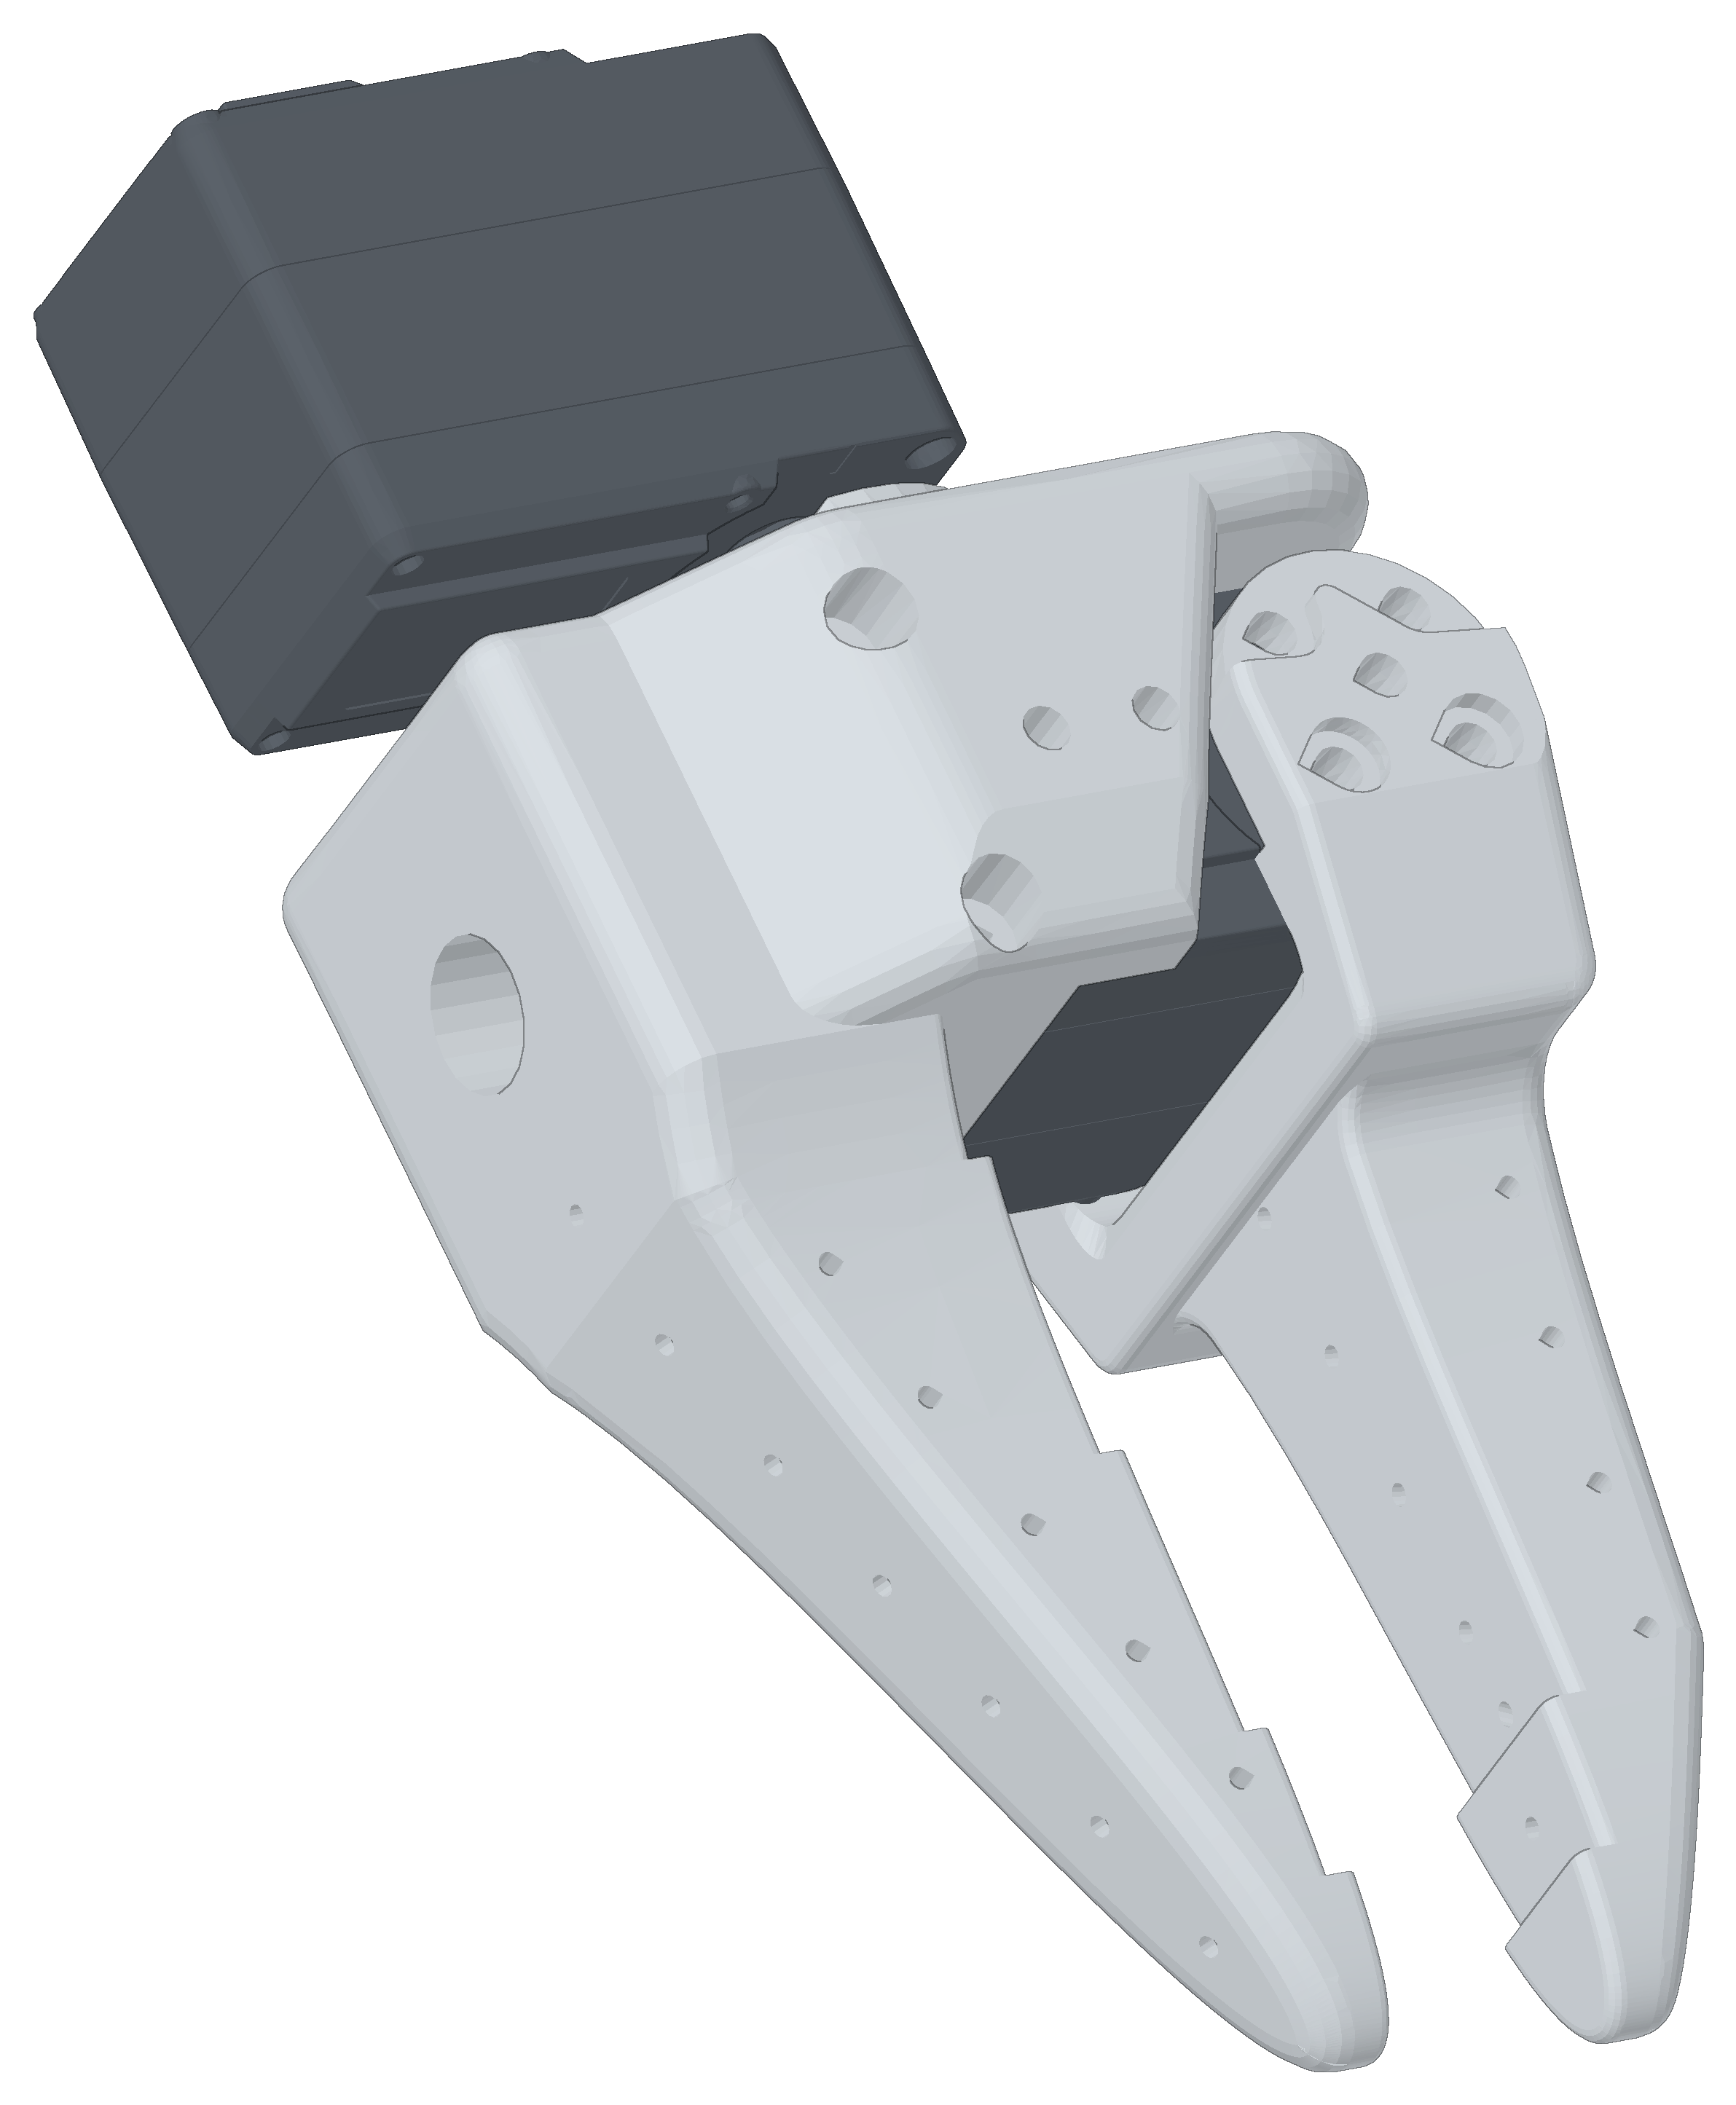
\includegraphics[width=0.65\linewidth,height=0.32\textheight,keepaspectratio]{images/cad-wrist-gripper-export.png}\par\medskip
\begin{tikzpicture}[x=0.13cm,y=0.55cm,>=Stealth,font=\small]
\fill[gray!20] (-4,0) rectangle (0,1.3);
\fill[gray!20] (65,0) rectangle (69,1.3);
\draw[thick] (0,0)--(0,1.3) (65,0)--(65,1.3);
\draw[fill=bluec!8,draw=bluec] (12.5,0.15) rectangle (52.5,1.1);
\node at (32.5,0.62) {40\,mm 工件};
\draw[<->] (0,1.8)--(65,1.8) node[midway,above] {$W_{\mathrm{open}}\approx65$\,mm};
\draw[<->] (0,-0.45)--(12.5,-0.45);
\draw[<->] (52.5,-0.45)--(65,-0.45);
\node[below] at (6.25,-0.45) {约12.5\,mm};
\node[below] at (58.75,-0.45) {约12.5\,mm};
\end{tikzpicture}
\caption{夹爪与腕部局部结构及工件进入余量}\label{fig:gripper-cad-clearance}
\end{figure}

上述数值受尺面倾斜、视差和遮挡影响，尚待现场读数复核；照片对应的舵机位置也未确认，不能直接作为抓取前 2619\,count 姿态的实测开口。工件偏转、定位误差和闭爪时序会改变实际进入条件，因此几何余量不能直接当作动态抓取容差。夹持状态由夹爪受阻后的位置反馈辅助判断，不等同于夹持力测量。

\subsubsection{电路各模块介绍}

本作品的电路以开发板与成品总线舵机为主，未自制电路板。信号链只有一级转接：可编程逻辑的
三态 IO 经一只总线转接板（出厂跳帽置 \code{Servo–TTL}）转成单线总线，六只舵机并联挂在
该总线上；舵机由独立的 5--14\,V 电源供电，与开发板共地。信号线共四根：\code{BUS\_TX}
（三态输出）、\code{BUS\_RX}（输入）、\code{BUS\_DIR}（换向控制，与三态使能同源）、
以及硬件\textbf{禁发}输入（跳线到地才允许发帧，拔掉立即中止）。换向时刻由硬件状态机保证，
不由软件延时决定，这是六轴能在同一帧内被广播、且不会互相踩线的直接原因。

信号与供电的连接关系见图~\ref{fig:wiring}。

\begin{figure}[H]\centering
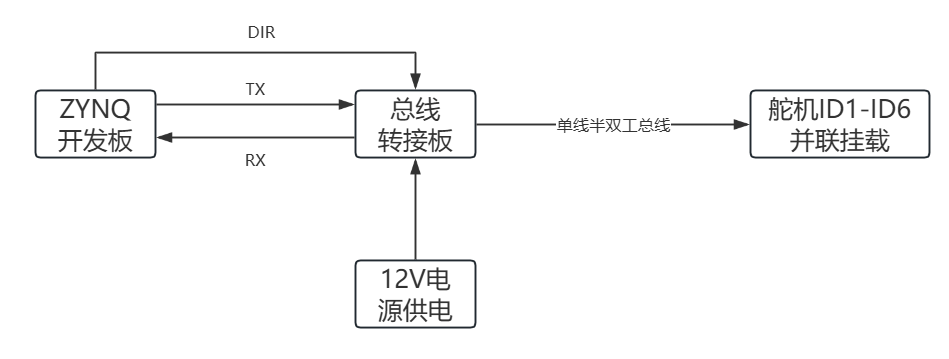
\includegraphics[width=\linewidth]{images/硬件.png}
\caption{信号与供电连接关系：三态 IO 的 TX/RX 与 DIR 经总线转接板（出厂跳帽置
Servo-TTL）并到一条单线半双工总线上，六只舵机并联挂载；舵机由独立电源 5--14\,V
供电，并与开发板共地}
\label{fig:wiring}
\end{figure}

\subsection{软件系统介绍}

\subsubsection{软件整体介绍}

软件总体分三层，分别为上位机、PS 和 PL。
\begin{table}[H]\centering\small
\caption{三层职责划分与关键实现}
\begin{tabularx}{\linewidth}{@{}p{1.5cm}p{2.4cm}Xp{4.0cm}@{}}
\toprule
层 & 载体 & 职责 & 关键实现 \\
\midrule
决策层 & 上位机 & 取帧、检测、平面映射、稳定判据、下发坐标、留存证据 & \code{capture\_agent.py}、\code{grasp\_point.py} \\
编排层 & PS（ARM Linux） & 坐标$\rightarrow$六轴目标（示教表插值）、七步状态机、夹持判定、故障恢复 & \code{grasp\_point\_map.py}、\code{g3\_station\_runner.py} \\
执行层 & PL（FPGA 逻辑） & 总线协议时序、六轴同步组帧、逐轴限位、deadline、故障锁存 & \code{src/pl/rtl/*.sv} \\
\bottomrule
\end{tabularx}
\end{table}

端到端的时间预算（实测，单轮 7.5--9.4\,s）见表~\ref{tab:timing}。

\begin{table}[H]\centering\small
\caption{单轮七步的分段耗时（13 次闭环实测）}
\label{tab:timing}
\begin{tabularx}{\linewidth}{@{}p{2.5cm}p{3.1cm}X@{}}
\toprule
阶段 & 典型耗时 & 说明 \\
\midrule
视觉出点 & 约 1.7\,s & 含预热丢弃帧与 0.5\,s 稳定窗，共 6--7 帧 \\
串口下发 + 校验 & $<$20\,ms & 单行约 200 字节，115200\,8N1 \\
approach & 0.88--4.21\,s & 首轮从复位位直接插值到抓取位，故偏长 \\
grasp + 闭爪 & 0.17\,s + 1.22\,s & 闭爪堵转耗时固定约 1.2\,s \\
lift & 0.83--0.99\,s & 六轴联动，ID1 锁定 \\
place + 张爪 & 1.85--2.20 + 0.66\,s & 先单轴 ID1 横摆，再六轴下放 \\
retreat + exit & 0.88\,s + 0.88\,s & 张爪后先垂直抬起再撤离 \\
\bottomrule
\end{tabularx}
\end{table}

连续抓取（模式一）的时间预算和静态完全不同。它把“等”换成了“算”，见
表~\ref{tab:timing2}。关键量是 $T_{\text{flight}}$：从触发帧到咬合的时间预算，
$T_{\text{flight}} = (x_{\text{int}} - x_{\text{trig}}) / v + (t_{\text{close}} + t_{\text{stage}})$
的余量必须为正，因此带速越高、检测线越要前移。

\begin{table}[H]\centering\small
\caption{模式一（连续抓取）的分段耗时，15 次命中实测}
\label{tab:timing2}
\begin{tabularx}{\linewidth}{@{}p{3.0cm}p{3.0cm}X@{}}
\toprule
阶段 & 实测 & 说明 \\
\midrule
视野现估带速 & 60.4--66.7\,mm/s & 最近 12 帧最小二乘，每轮重算 \\
飞行时间 $T_{\text{flight}}$ & 3.39--3.80\,s & 由当帧 $x$ 与拦截点 350\,mm 反算 \\
臂推进 & \textbf{1952}\,ms & 从待命位（撤离位高点）到拦截点，六轴插值 \\
到位抖动 & \textbf{4--19}\,ms & 折合 0.25--1.2\,mm，与落点偏差同量级 \\
闭爪→咬合 & \textbf{1010}\,ms & 夹住时卡在接触位、等满观测窗 \\
搬运往返 & 约 1.6\,s & lift→place→retreat→exit \\
\midrule
抓取段合计 & P50 \textbf{4589}\,ms & P95 4788\,ms，max 5458\,ms；不含视觉出点与回待命位，完整一轮 P50 8.6\,s \\
\bottomrule
\end{tabularx}
\end{table}

\subsubsection{软件各模块介绍}

\paragraph{（一）上位机：取点与稳定判据}

主流程为：打开相机 $\rightarrow$ 丢弃预热帧 $\rightarrow$ 连续检测取中位数
$\rightarrow$ 稳定判据 $\rightarrow$ 平面映射 $\rightarrow$ 下发。关键输入为图像帧与
标定文件，关键输出为一对毫米坐标与一组证据字段（帧数、极差、置信度、带面重合度）。

\textbf{稳定判据}是本模块的核心。设最近 $n$ 帧中心为 $c_1 \ldots c_n$，当且仅当
$\max x - \min x \leq 2$\,mm、$\max y - \min y \leq 2$\,mm 且首末帧时间跨度
$\geq 0.5$\,s 时，取中位数作为出点；达不到门槛就不出点，继续采样到超时，并在日志里
打出当前极差（\code{CAPTURE\_WARN}）。

\textbf{平面映射}采用四点单应：在带面四角取像素点，与 490\,mm$\times$80\,mm 的物理尺寸
建立透视变换，像素经一次矩阵乘法得毫米坐标。标定由程序自动完成（HSV 绿掩膜 + 最小外接
矩形找带四角），人工只需确认一次。

\textbf{误检治理}分三级：算法（只用带面四边形内的检测框，框外的夹爪误检点直接被排除）、
选点（框内按 $x$ 从大到小取最下游一件，已抓过的位置先剔除，避免同一件重复触发）、
判据（置信度门槛另设一道，并记录 top1 与 top2 的差值，差值过小则告警）。

\paragraph{（二）PS：坐标到关节，以及七步状态机}

\textbf{坐标$\rightarrow$关节}用六点五轴示教表分段线性插值，表中每点为 $(x,y)$ 与五个
关节目标值，实测值见表~\ref{tab:teach}。

\begin{table}[H]\centering\small
\caption{六点示教表（$y=36$\,mm ，单位：舵机 count，范围0-4000）}
\label{tab:teach}
\begin{tabular}{@{}crrrrr@{}}
\toprule
$x$ / mm & ID1 & ID2 & ID3 & ID4 & ID5 \\
\midrule
295 & 1699 & 2109 & 2141 & 2923 & 1687 \\
320 & 1806 & 2030 & 2226 & 2885 & 1706 \\
345 & 1854 & 2010 & 2241 & 2942 & 1757 \\
370 & 1937 & 1971 & 2296 & 2972 & 1845 \\
395 & 2039 & 1965 & 2287 & 2932 & 1950 \\
420 & 2185 & 1912 & 2369 & 2873 & 2107 \\
\bottomrule
\end{tabular}
\end{table}

\textbf{七步状态机}的流程与出口条件见图~\ref{fig:steps}。其中三条约束是为解决碰撞问题
而加的：抬升段必须六轴联动，因为第二关节单独动作时，接近竖直位会因低速死区停在中途，
末端姿态随之失控；离地之前不许横向移动，横移一律交给放置段；带件横摆必须保持高位，
先单轴摆到位再六轴下放。此外抬升与放置期间两只腕关节必须同步跟随，否则腕部自转会使
工件相对夹爪转动而脱落。

\begin{figure}[H]\centering
\begin{tikzpicture}[
  st/.style={draw,rounded corners=2pt,fill=blue!6,align=center,inner sep=2.4pt,
             font=\scriptsize,minimum height=11mm,text width=17mm},
  ar/.style={-{Latex[length=1.5mm]},draw=bluec}]
% 第一行（左->右）
\node[st] (s1) at (0,0)      {standby\\归循环位};
\node[st] (s2) at (2.15,0)   {approach\\六轴插值};
\node[st] (s3) at (4.30,0)   {grasp\\落到抓取位};
\node[st] (s4) at (6.45,0)   {grasp.gripper\\闭合判夹持};
\node[st] (s5) at (8.60,0)   {lift\\六轴联动\\ID1 锁定};
% 第二行（右->左）
\node[st] (s6) at (8.60,-2.1) {place\\先单轴横摆\\再六轴下放};
\node[st] (s7) at (6.45,-2.1) {place.gripper\\张开};
\node[st] (s8) at (4.30,-2.1) {retreat\\先垂直抬\\再横移};
\node[st] (s9) at (2.15,-2.1) {exit\\回撤离位};
\draw[ar] (s1)--(s2); \draw[ar] (s2)--(s3); \draw[ar] (s3)--(s4); \draw[ar] (s4)--(s5);
\draw[ar] (s5)--(s6); \draw[ar] (s6)--(s7); \draw[ar] (s7)--(s8); \draw[ar] (s8)--(s9);
\end{tikzpicture}
\caption{七步状态机流程（grasp.gripper 与 place.gripper 为夹爪动作子步）}
\label{fig:steps}
\end{figure}

\textbf{夹持判定}读舵机闭合并堵转后的位置：命令目标为 2200，实际停在 2373--2409
说明夹住了工件（差 170+ count），停到 2214 说明合到底、没夹到东西，阈值取 60 count。
这条判据让“七步全绿但没夹到东西”的假成功无法进入统计。

\textbf{七步是执行层的骨架，两种模式共用同一套。}静态时七步一次走完，何时开始由操作者
决定；连续抓取时，前两步换成“按预测时刻推进”，从 grasp 起的后五步原样复用。模式一没有
另写一套动作，只是给同一套动作换了个触发方式。好处很实在：动作序列只调一次、两处共用，
搬运段那几条为避碰撞定下的约束（抬升必须联动、离地之前不许横移、带件横摆要保持高位）
对两种模式同时生效，调好一个就是两个都好，模式二的验收也顺带覆盖了模式一的后半段。
代价同样写在明处：夹取姿态不随视觉实时修正，误差只能靠标定与示教在前面压住，这条边界
见 \S 4.2。

\paragraph{（三）动态触发：预测拦截}

连续抓取要在时机上动手，\textbf{把“等工件”换成“算工件”}，动作本身并没有更快。模块输入是每帧
检测框与时间戳，输出是一个“何时、去哪”的动作：异常件越过触发线后，先以最近若干帧的
位移做最小二乘拟合得到当前带速 $v$，再由飞行时间反算本轮拦截点

\begin{equation}
x_{\text{int}} = x_{\text{trig}} + v \cdot (t_{\text{adv}} + t_{\text{move}} + t_{\text{margin}}),
\qquad
T_{\text{flight}} = \frac{x_{\text{int}} - x_{\text{trig}}}{v} + t_{\text{close}} + t_{\text{stage}}
\end{equation}

其中臂推进 $t_{\text{stage}}$ 实测 1952\,ms、闭爪 $t_{\text{close}}$ 实测 1010\,ms、
推进余量 $t_{\text{margin}}$ 取 300\,ms。时序关系见图~\ref{fig:timeline}：臂在
$T_{\text{flight}}$ 期间停在待命位，到点才向 $x_{\text{int}}$ 推进，\textbf{到位即闭爪}，
不在固定点上提前等着。

\begin{figure}[H]\centering
\begin{tikzpicture}[x=1mm,y=1mm,font=\scriptsize]
% 时间轴
\draw[-{Latex[length=2mm]},thick] (0,0) -- (100,0) node[below left,font=\tiny]{时间};
% 触发 / 咬合 两条时刻线
\draw[dashed,bluec] (8,-2) -- (8,20);
\node[bluec,font=\tiny,above] at (8,20) {触发};
\draw[dashed,red!70!black] (86,-2) -- (86,20);
\node[red!70!black,font=\tiny,above] at (86,20) {咬合};
% 两段耗时
\fill[blue!22] (8,4) rectangle (58,10);
\node at (33,7) {臂推进 1952\,ms};
\fill[orange!30] (58,4) rectangle (86,10);
\node at (72,7) {闭爪 1010\,ms};
% 工件位移（即 T_flight 预算）
\draw[{Latex[length=1.6mm]}-{Latex[length=1.6mm]},thick,green!42!black] (8,15) -- (86,15)
  node[midway,above,font=\tiny]{$T_{\text{flight}}$ 预算（工件位移）};
% 对齐说明
\draw[gray,dotted] (8,10) -- (8,13.4);
\draw[gray,dotted] (58,10) -- (58,4);
\end{tikzpicture}
\caption{连续抓取的时间轴：触发后按预算推进，臂到位与工件到位同时发生，随即闭爪咬合}
\label{fig:timeline}
\end{figure}

这个“到点推进、到位即闭爪”的形态是两版方案对比后的选择：早期版本让机械臂提前停在固定
拦截点，工件须从张开的夹爪开口中自行走过约 57\,mm，横向偏移稍大就会被夹指挡住；改为按
预测时刻推进后，工件在开口内的行程缩短到约 23\,mm，命中率由 69\%（9/13）提升到
93.8\%（15/16）。

另有两条约束写死在参数里。一条是\textbf{触发线要足够靠前}，取 $x=120$\,mm，须满足
$x_{\text{trig}} \le x_{\text{int}} - v \cdot (t_{\text{stage}} + t_{\text{close}})$，
按 60--67\,mm/s 折算需要 180--200\,mm 的间距，现取 230\,mm，余量只有 30--50\,mm；
带速再高就必须把触发线继续前移或进一步缩短臂行程；
另一条是\textbf{夹持判据要提前}，闭爪耗时约 1010\,ms 对应“夹住”，约 560\,ms 对应“空夹”，
比读回接触位置早一整轮，可当场决定是否重试，而不必等搬运结束。

\paragraph{（四）PL：总线时序与安全校验}

PL 侧模块划分与职责见表~\ref{tab:pl}。

\begin{table}[H]\centering\small
\caption{PL 模块划分（合计 2100+ 行 SystemVerilog）}
\label{tab:pl}
\begin{tabular}{@{}p{5.1cm}rp{4.9cm}@{}}
\toprule
模块 & 行数 & 职责 \\
\midrule
\code{hx30hm\_g1\_engine.sv} & 295 & 半双工单线协议：组帧、校验、换向时序 \\
\code{servo\_bus\_master.sv} & 72 & 总线占用与仲裁 \\
\code{g2\_six\_axis\_controller.sv} & 443 & 六轴同步组帧、逐轴到位判定、限位、速度上限、deadline、标定日志 \\
\code{g2\_descriptor\_guard.sv} & 71 & 命令描述符硬校验，非法帧在进总线前被拒 \\
\code{safety\_monitor.sv} & 13 & 急停/看门狗/协议故障锁存，门控 \code{motion\_permit} \\
\code{axi\_lite\_regs.sv} + \code{rtcs\_pkg.sv} & -- & ABI \code{0x5254000E} 寄存器映射 \\
\code{trajectory\_engine.sv} & 15 & 接口预留，当前不产生运动（边界见 4.2 节） \\
\bottomrule
\end{tabular}
\end{table}

三类安全机制都在 PL 内实现：\textbf{逐轴限位}在组帧前比对实测限位表，越界帧直接拒绝；
\textbf{截止时间校验}为每条命令设 deadline，超时标记 \code{deadline\_miss} 并回报而不
阻塞后续命令；\textbf{故障锁存}把舵机错误位分轴保存，配合掩码区分“可屏蔽的过载”与
“不可屏蔽的通讯/限位故障”。之所以放在 PL：这些判断必须在帧发出前的同一拍完成，
放到 Linux 侧就会受调度延迟影响。

% =============================================================================
\section{完成情况及性能参数}

\subsection{整体介绍}
系统以输送带、机械臂、俯视相机及控制板构成桌面视觉分拣工位。输送带水平布置，机械臂固定在带侧，末端夹爪由侧方进入带面上方；相机通过独立支架安装在输送带上方，用于观测工件位置。上位机承担视觉处理，控制板连接机械臂执行端，形成从视觉观测到抓取执行的工位布局。

图~\ref{fig:mechanical-real-layout} 为工位正面实拍，图~\ref{fig:workstation-oblique} 展示斜侧安装关系，图~\ref{fig:workstation-overhead} 补充俯视布局。三种视角共同展示相机支架、输送带、机械臂与控制板的位置关系。斜侧与俯视照片对背景海报、人物作了清理，原始照片另行保留；照片用于说明工位布局，不作为尺寸测量依据。
\begin{figure}[H]\centering
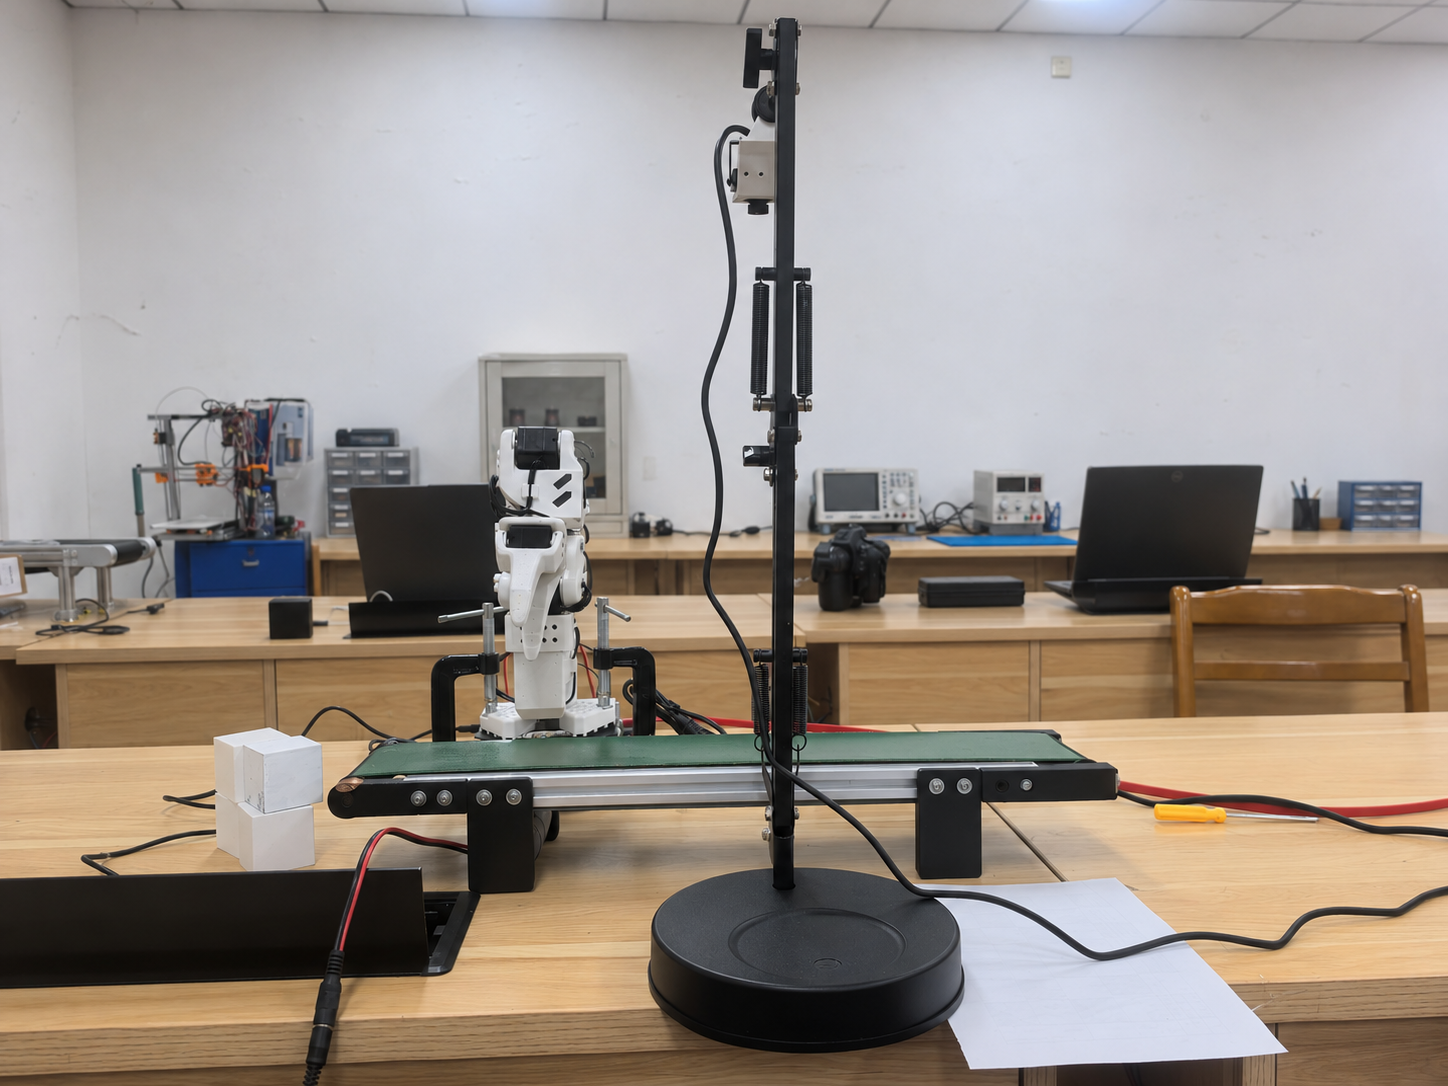
\includegraphics[width=0.96\linewidth,height=0.40\textheight,keepaspectratio]{images/workstation-front-original.jpg}
\caption{视觉分拣工位正面实拍}\label{fig:mechanical-real-layout}
\end{figure}
\begin{figure}[H]\centering
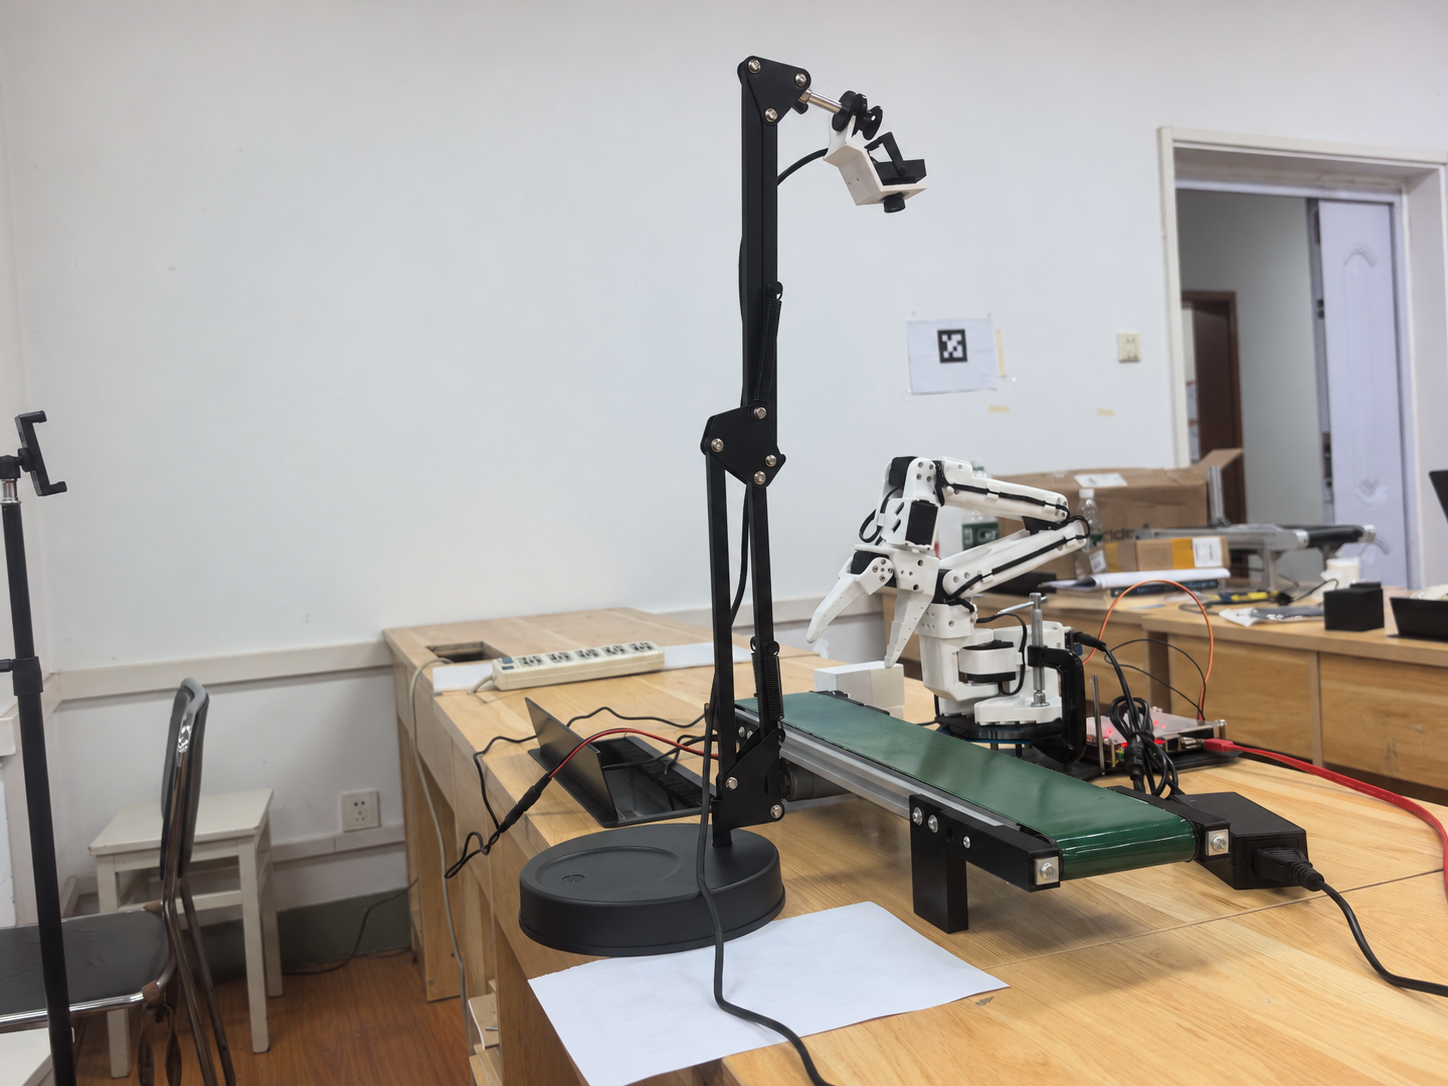
\includegraphics[width=0.96\linewidth,height=0.40\textheight,keepaspectratio]{images/workstation-oblique-natural-cleanup.png}
\caption{工位斜侧全景（背景经清理）}\label{fig:workstation-oblique}
\end{figure}
\begin{figure}[H]\centering
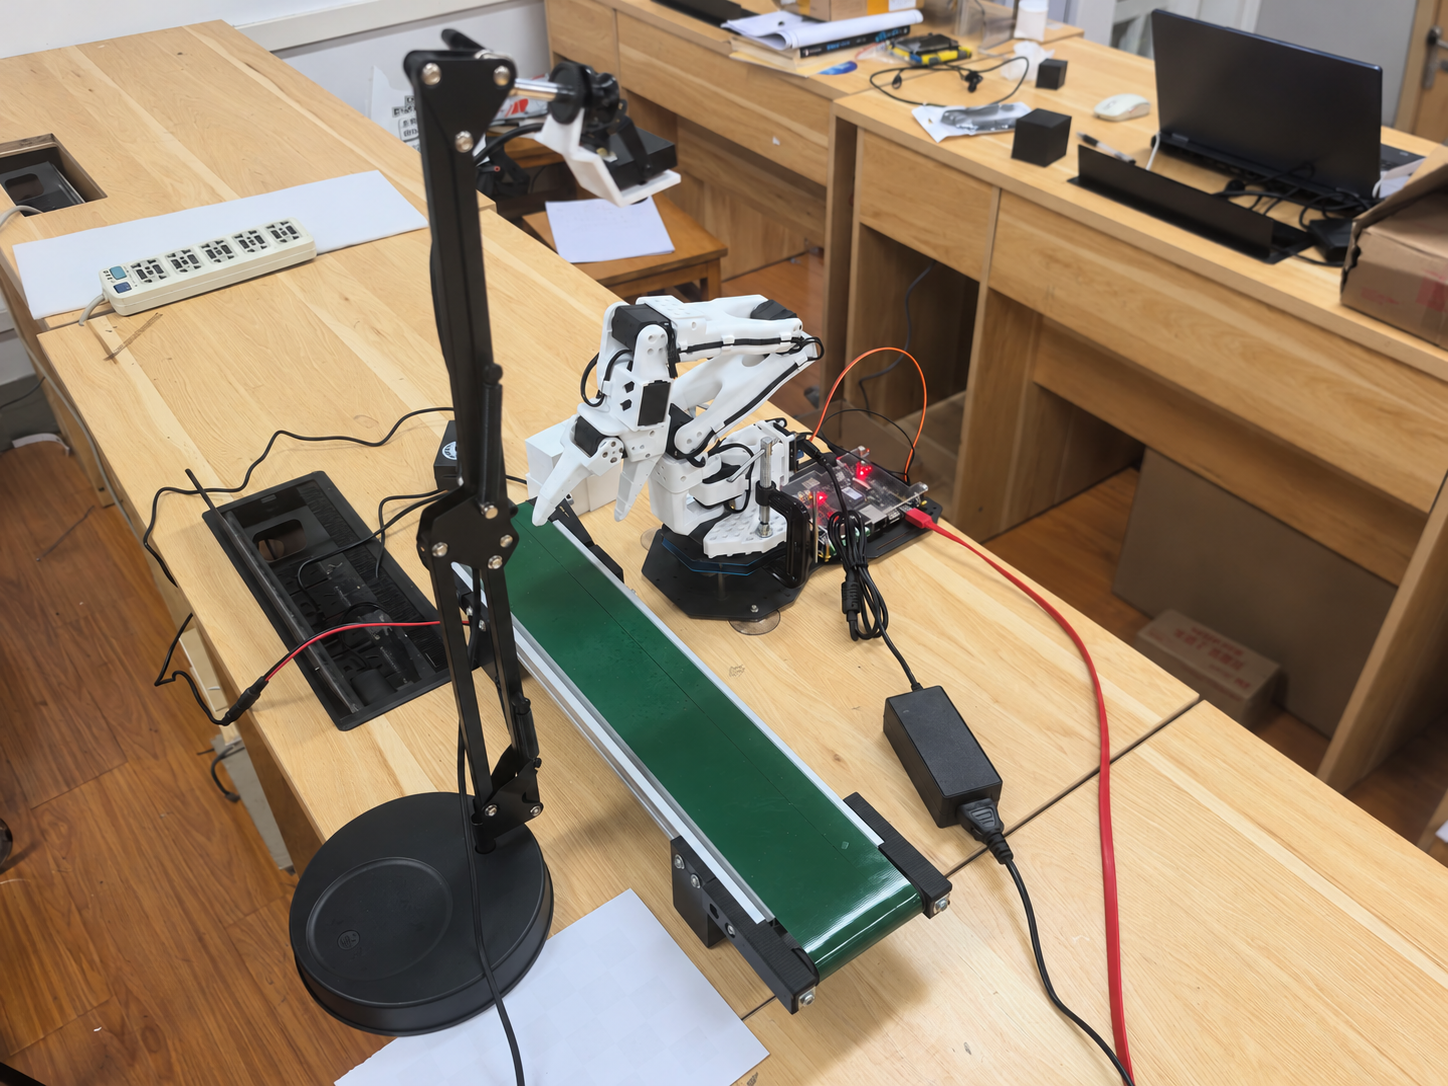
\includegraphics[width=0.96\linewidth,height=0.40\textheight,keepaspectratio]{images/workstation-overhead-natural-cleanup.png}
\caption{工位俯视布局（背景经清理）}\label{fig:workstation-overhead}
\end{figure}

\subsection{工程成果}
\subsubsection{机械成果}
机械臂、末端夹爪和基座固定组件已完成工位安装。工位正面与俯视布局见图~\ref{fig:mechanical-real-layout} 和图~\ref{fig:workstation-overhead}，机械臂侧面近景见图~\ref{fig:mechanical-real-arm}；侧面视角补充展示连杆、腕部夹爪及基座夹紧关系。白色结构件连接关节与臂段，末端两指夹爪处于张开状态；底部通过支承底板及螺杆夹紧组件固定于工作台。舵机线束沿臂段外侧布置，并在关节附近保留活动余量。照片能够展示机构组成与固定方式，但不能据此给出夹爪开口或连杆长度的测量结果。
\begin{figure}[H]\centering
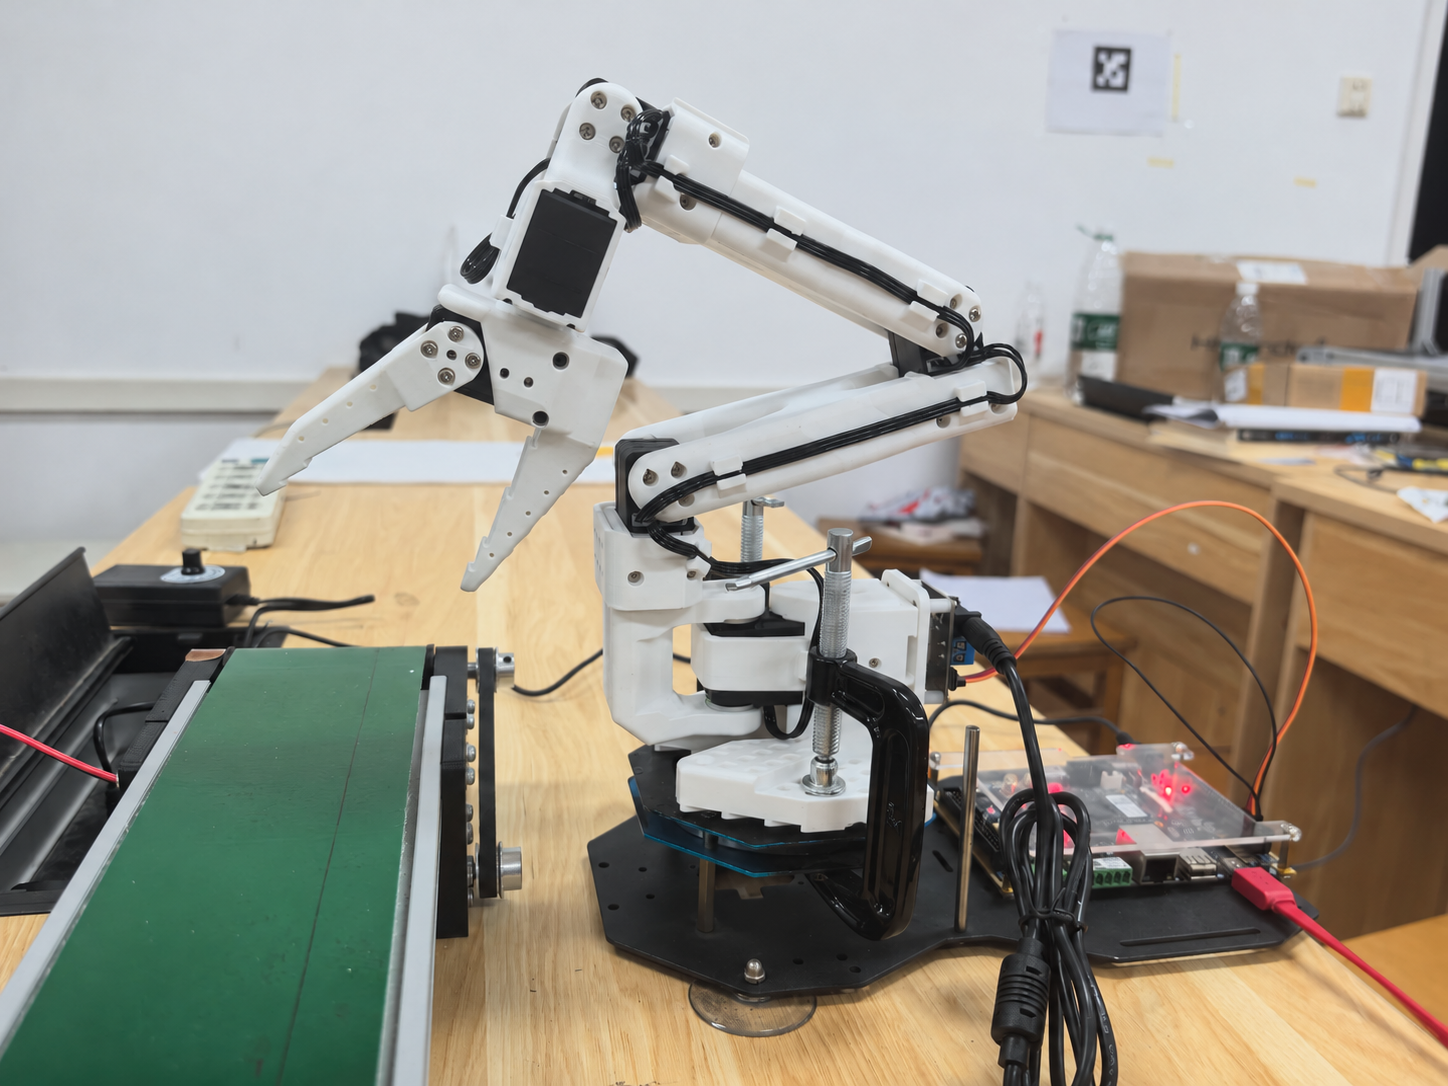
\includegraphics[width=0.92\linewidth,height=0.38\textheight,keepaspectratio]{images/robot-closeup-poster-removed.png}
\caption{机械臂侧面近景：连杆、张开夹爪与基座固定（背景海报已去除）}\label{fig:mechanical-real-arm}
\end{figure}
\begin{figure}[H]\centering
\begin{minipage}[t]{0.48\linewidth}\centering
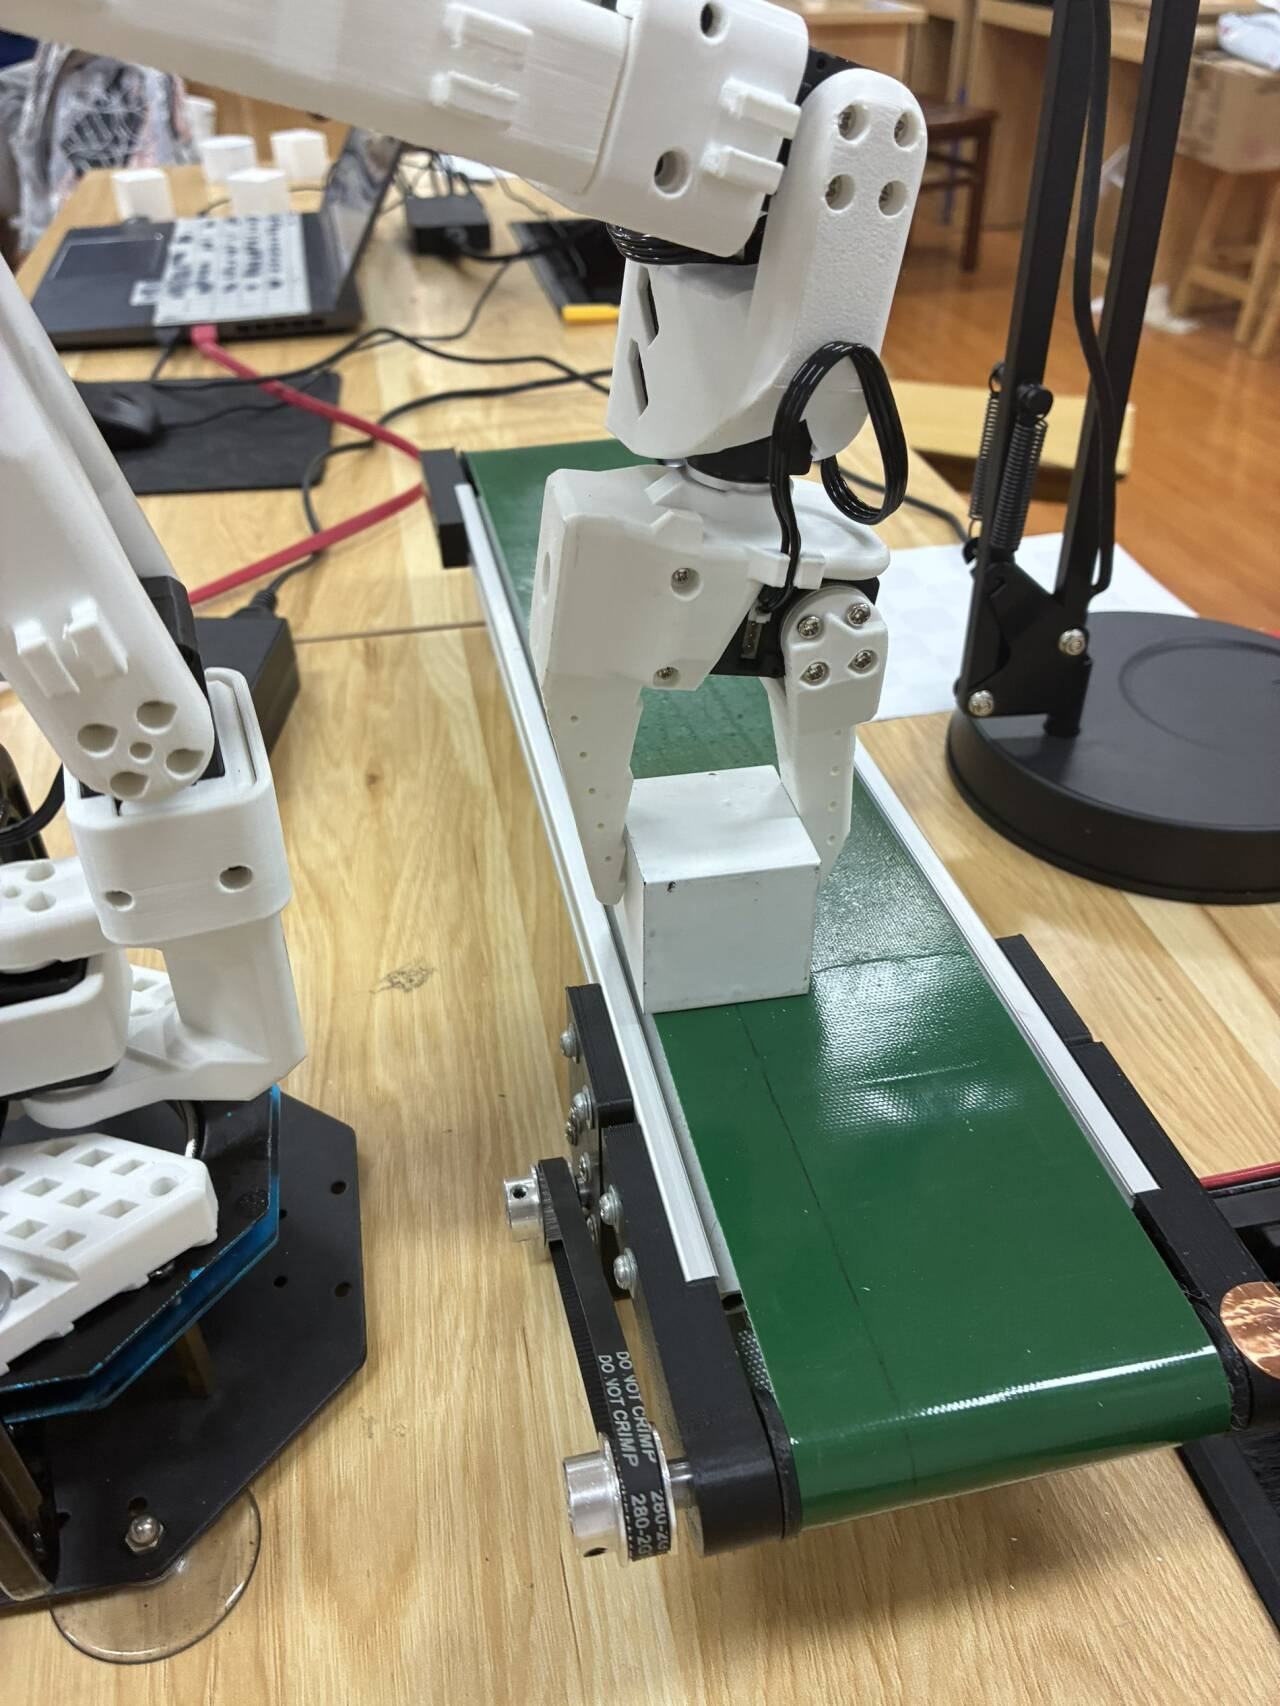
\includegraphics[width=\linewidth,height=0.42\textheight,keepaspectratio]{images/gripper-closed-portrait.png}
\par\smallskip{\small （a）夹爪收拢状态}
\end{minipage}\hfill
\begin{minipage}[t]{0.48\linewidth}\centering
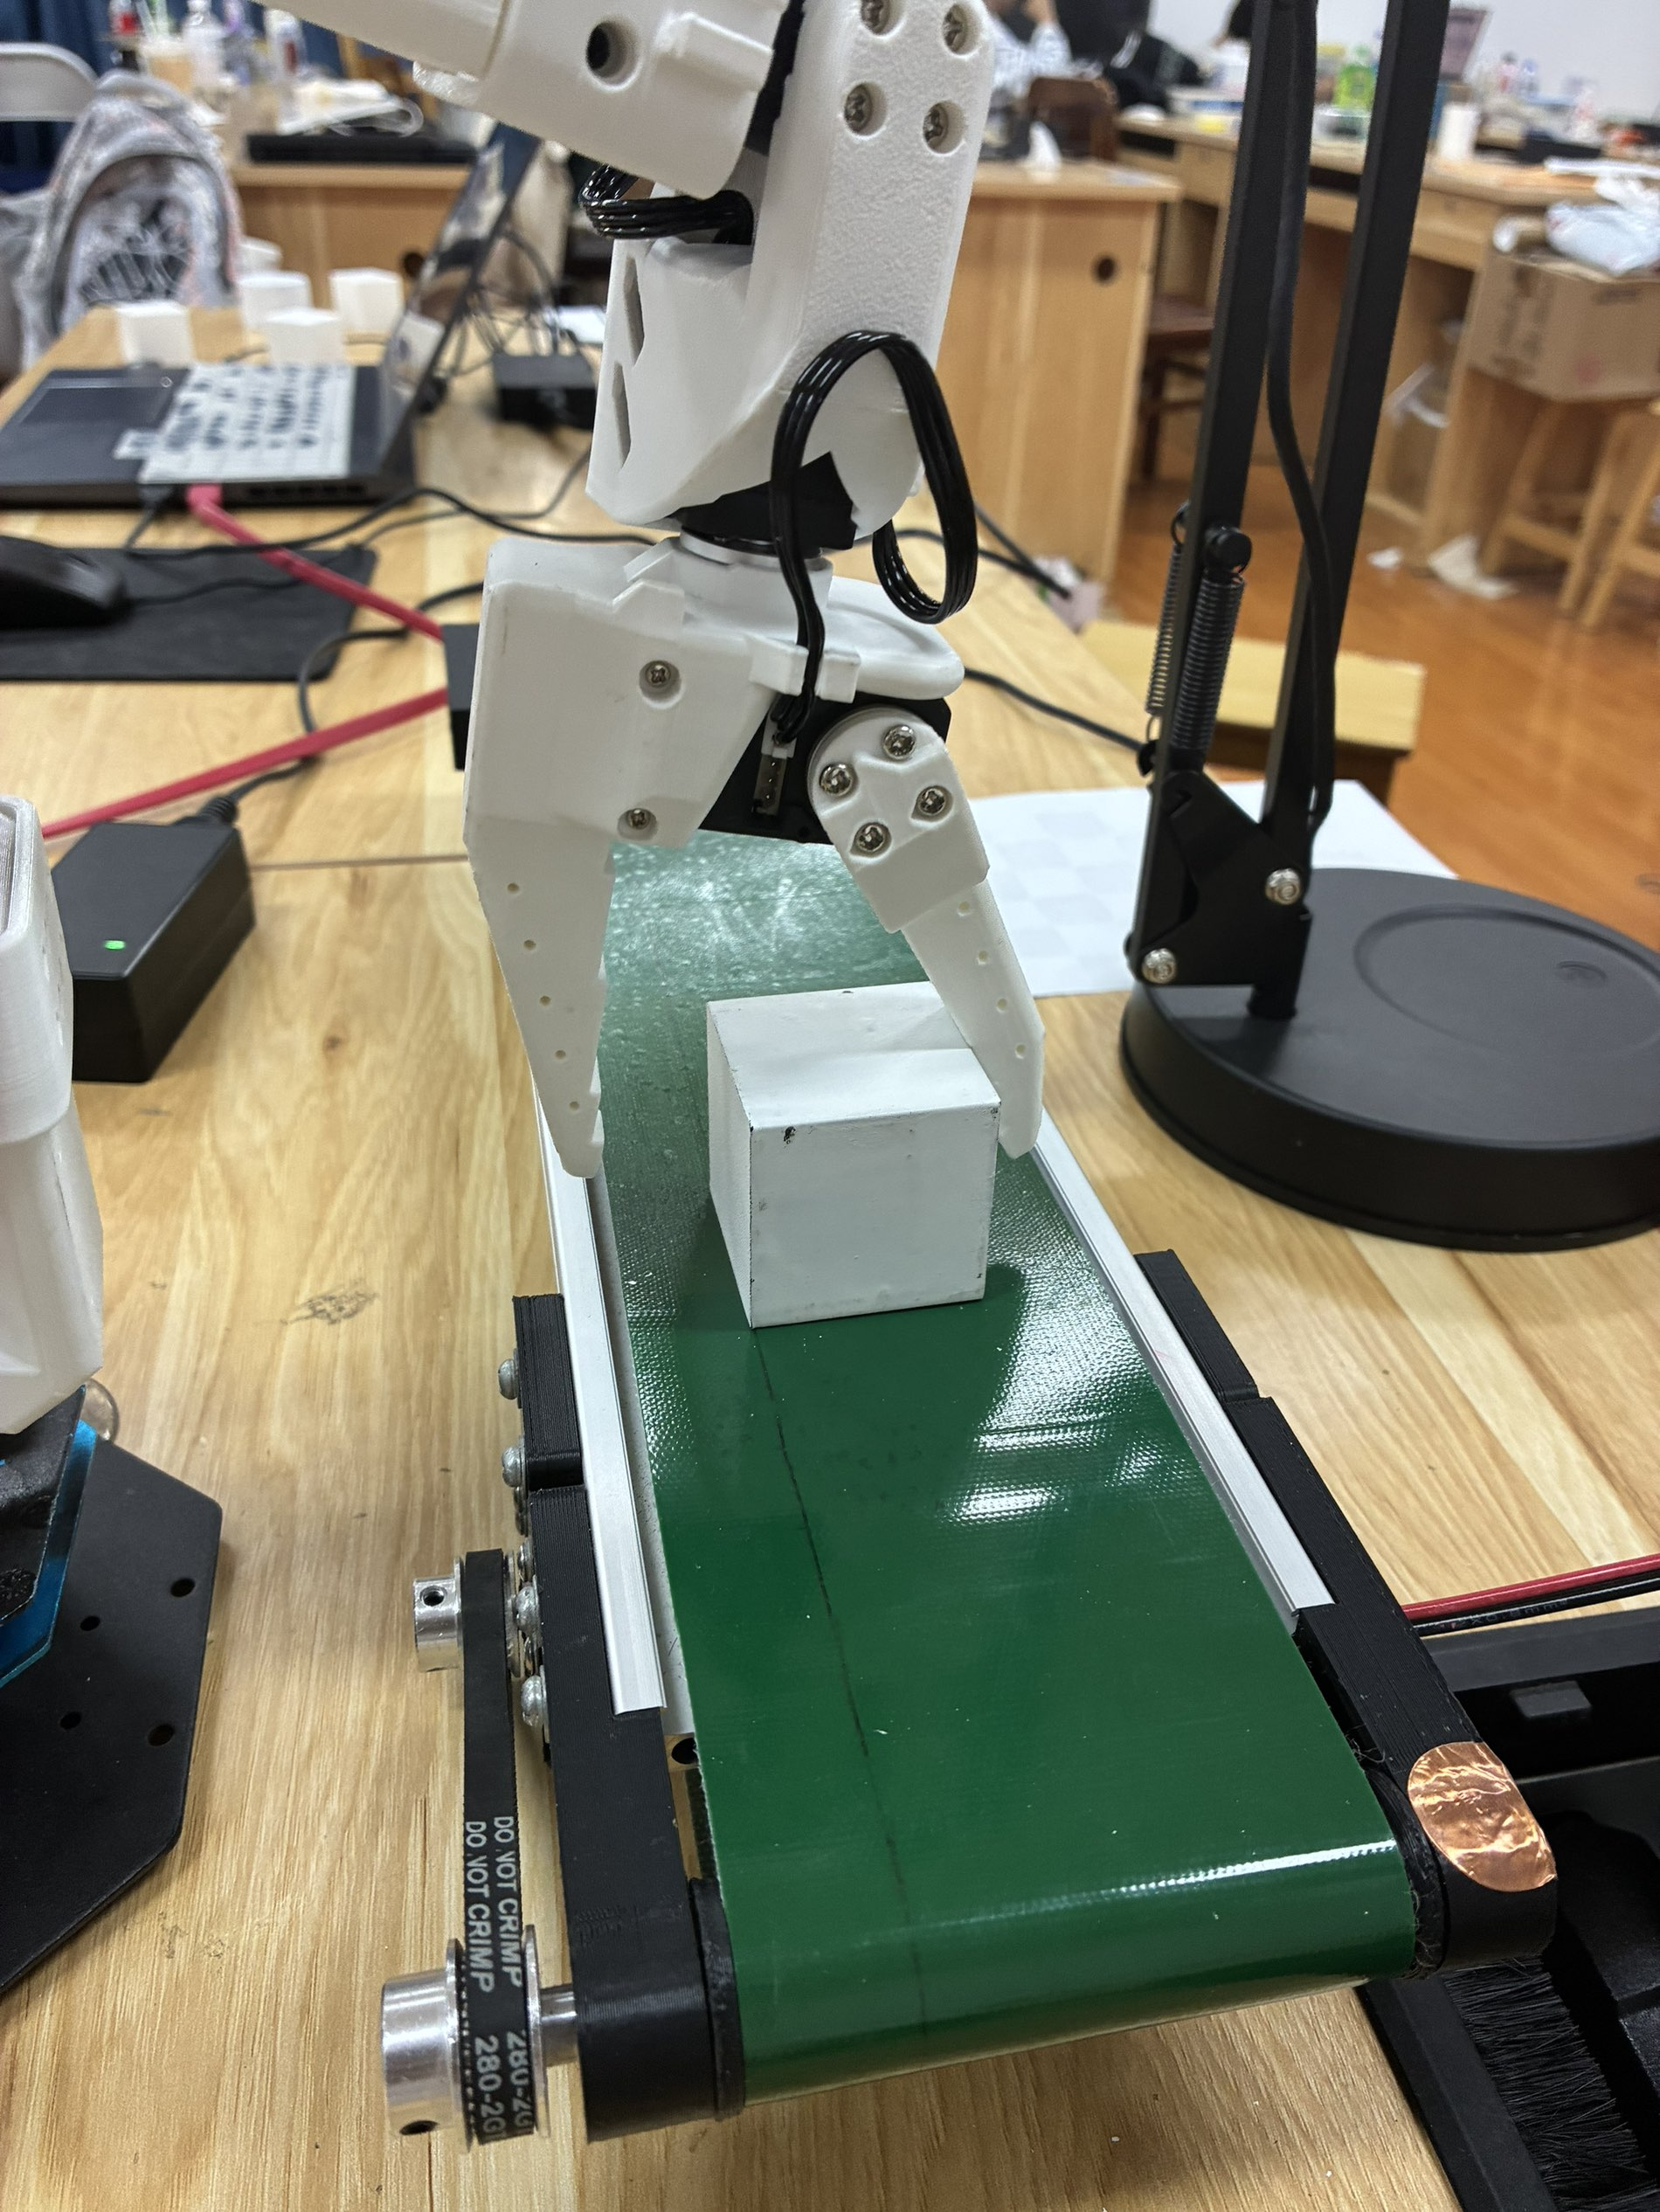
\includegraphics[width=\linewidth,height=0.42\textheight,keepaspectratio]{images/gripper-open-portrait.png}
\par\smallskip{\small （b）夹爪张开状态}
\end{minipage}
\caption{夹爪与方块工件的收拢、张开状态实拍}\label{fig:gripper-state-photos}
\end{figure}
图~\ref{fig:gripper-state-photos} 展示两指与工件的相对位置。收拢照片中工件仍位于带面上，照片用于说明夹爪状态，不据此单独判定已经夹牢或完成提起；两张照片均未提供尺面读数，不能用于确认有效开口的毫米数值。

\subsubsection{电路成果}
本作品采用开发板、总线转接板和独立舵机供电，未自制 PCB。电气连接原理见图~\ref{fig:wiring}，控制板、外部供电与机械臂的现场布局见图~\ref{fig:workstation-overhead}；机械臂侧面照片（图~\ref{fig:mechanical-real-arm}）也展示了基座旁控制板与线束的相对位置。上述全景用于说明安装布局，总线转接板的接口定义与逐线连接关系见图~\ref{fig:buslinker}。

总线转接板为幻尔 BusLinker-V3.0，板载 TTL 侧三针排针与上位信号对应：\code{BUS\_TX}
接 PL 输出、\code{BUS\_RX} 接 PL 输入、\code{GND} 与开发板共地；板载两路 S 端口用于
串接舵机总线，电源由蓝色接线端子引入，丝印标注上限 14\,V。该板出厂跳帽置于
\code{Servo}--\code{TTL} 档，即把 PL 的三态 IO 转换为单线半双工舵机总线；跳帽若误置
\code{USB} 档，总线将由板载 USB 芯片驱动而使 PL 失去控制权。
\begin{figure}[H]\centering
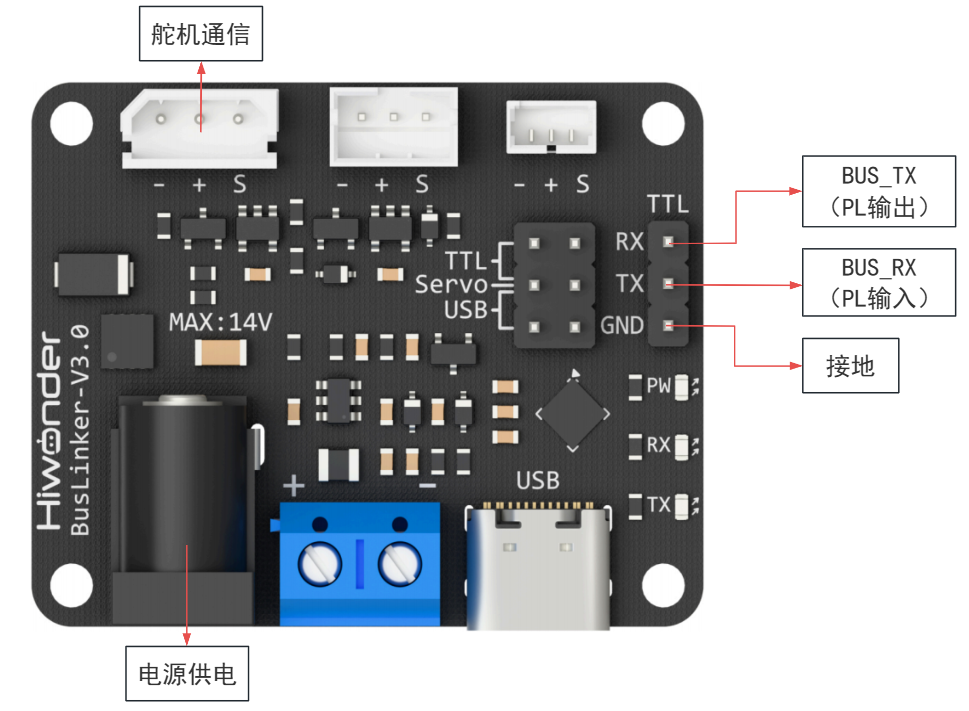
\includegraphics[width=0.85\linewidth,keepaspectratio]{images/PCB图.png}
\caption{总线转接板（BusLinker-V3.0）接口定义：TTL 侧 \code{BUS\_TX}/\code{BUS\_RX}/\code{GND}
对应 PL 输出、输入与共地，两路 S 端口串接舵机总线，电源经接线端子引入（上限 14\,V）}
\label{fig:buslinker}
\end{figure}

\subsubsection{软件成果}
视觉检测与带面坐标映射界面如图~\ref{fig:vision-detection-runtime} 所示。绿色框、中心点及文字展示方块的检测位置、类别与置信度，黄色四边形标出带面标定边界，界面同时输出映射后的 $X$、$Y$ 坐标。截图中两个方块的检测置信度分别为 0.84 和 0.80，界面显示 CPU 运行及瞬时帧率 22.6\,FPS；该值仅对应截取时刻，不作为完整测试的平均帧率。单帧界面用于展示检测和定位输出，不单独证明毫米定位精度或抓取成功率。
\begin{figure}[H]\centering
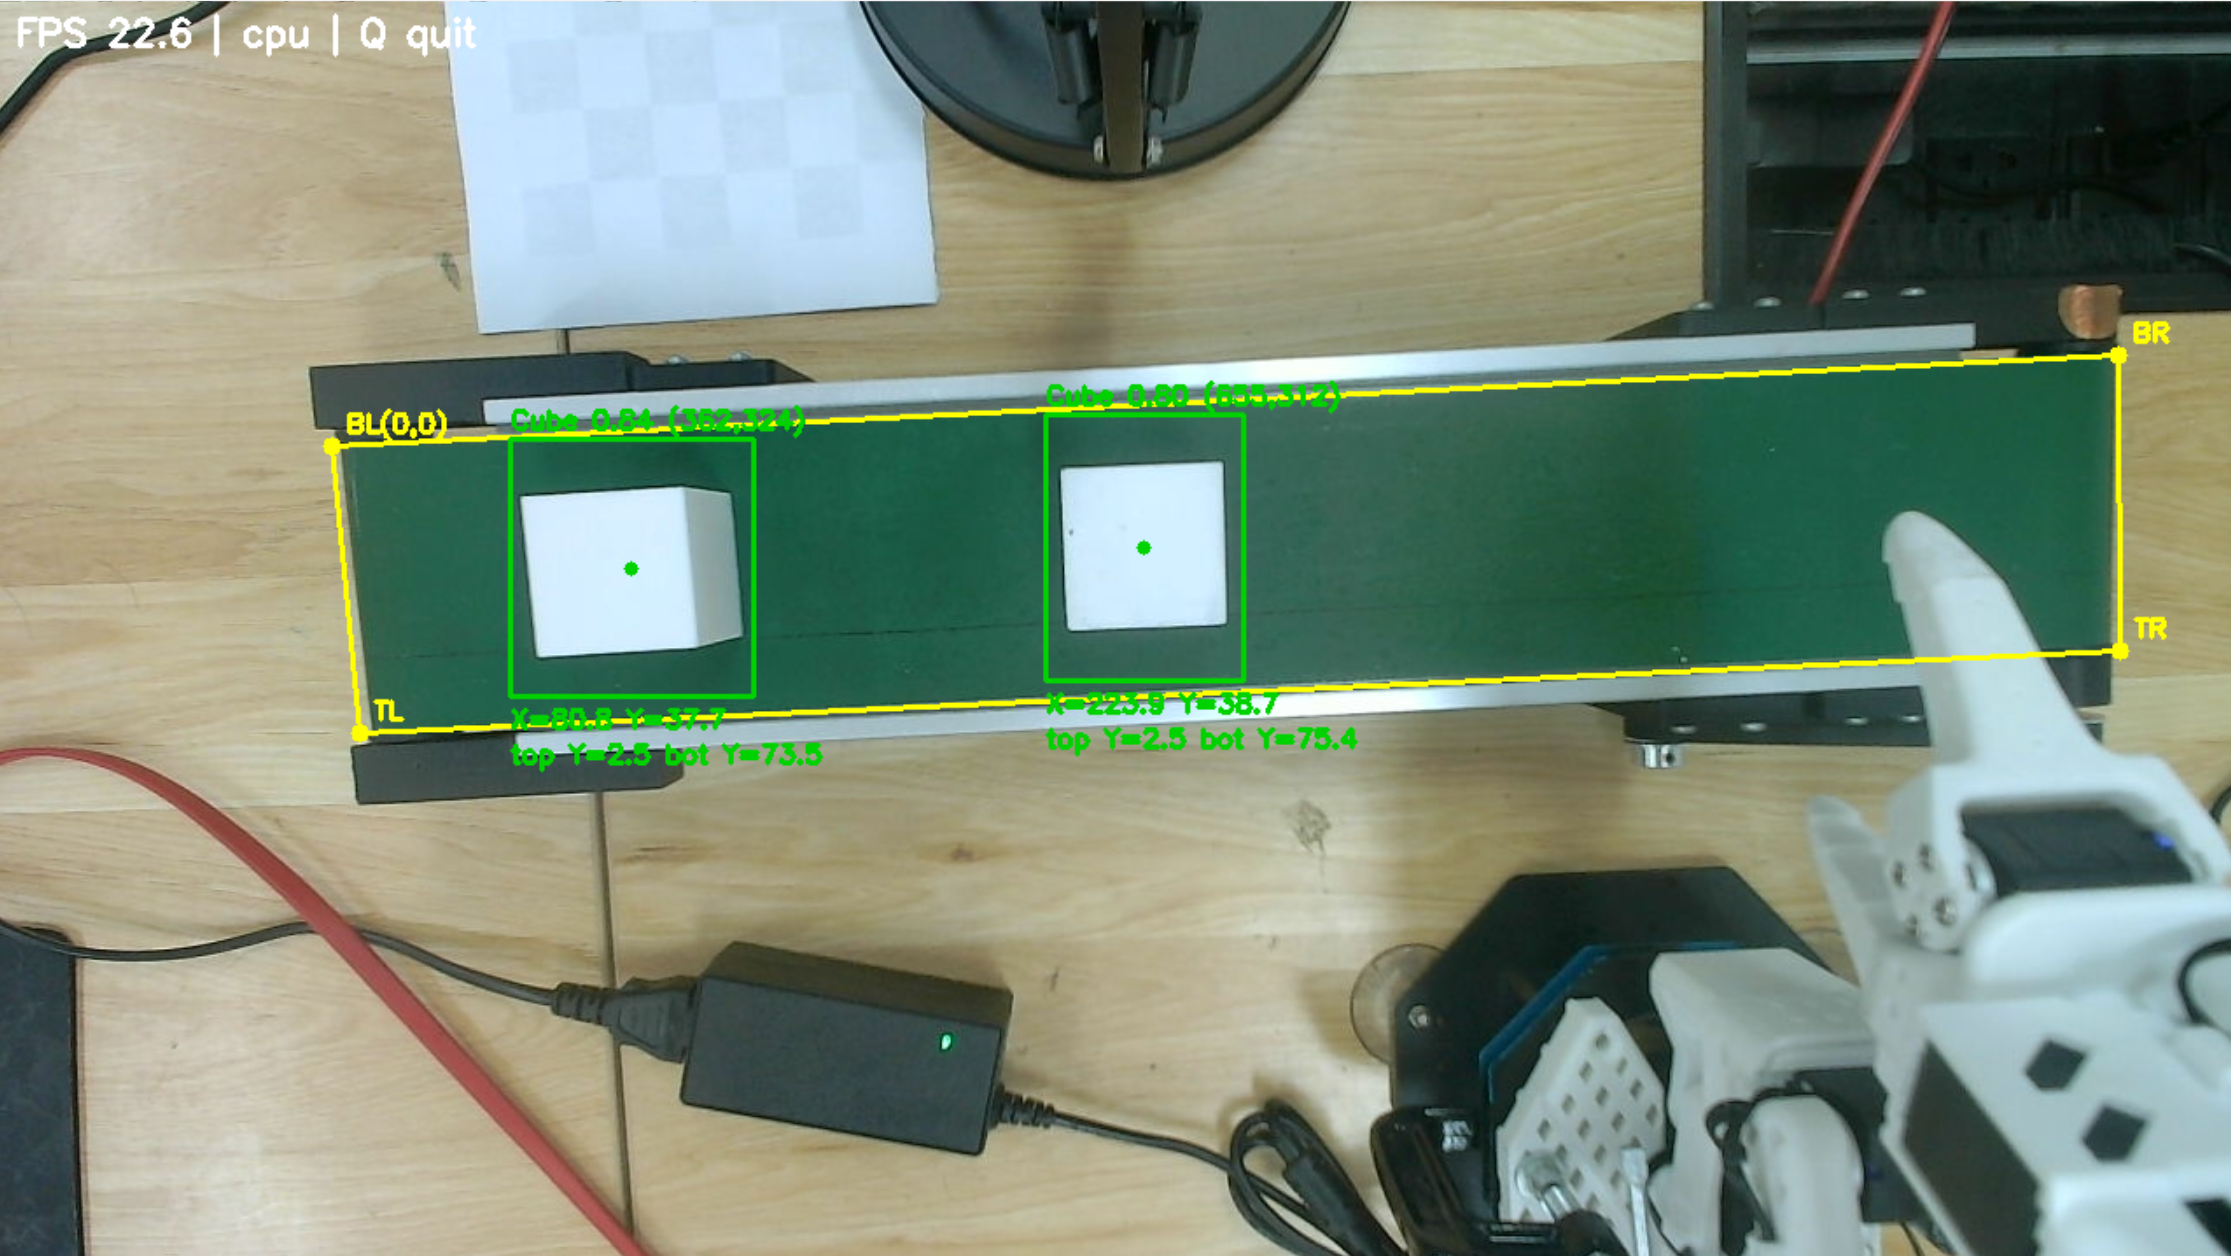
\includegraphics[width=\linewidth]{images/vision-detection-plane-mapping.png}
\caption{视觉检测与带面坐标映射运行界面}\label{fig:vision-detection-runtime}
\end{figure}

\subsection{特性成果}

\paragraph{（1）批次拣选闭环} 输送带静止、仅对异常类下发指令；13 次连续触发全部成功
抓取并放置，无碰撞、无掉件、无中途停滞。逐次记录见表~\ref{tab:trials}，原始日志与带框图随作品提交。

\begin{table}[H]\centering\footnotesize
\caption{静态抓取闭环逐次结果（2026-10-26，13 次连续触发）}
\label{tab:trials}
\begin{tabular}{@{}crrcccc@{}}
\toprule
\# & $x$ / mm & $y$ / mm & 夹持位置 & 周期 / ms & 判据 & 结果 \\
\midrule
1  & 372.16 & 36.13 & 2389 & 10961 & contact & 成功（首轮含归位） \\
2  & 357.62 & 35.79 & 2373 & 7741  & contact & 成功 \\
3  & 307.34 & 35.78 & 2409 & 8046  & contact & 成功 \\
4  & 341.86 & 37.63 & 2375 & 7843  & contact & 成功 \\
5  & 380.88 & 37.27 & 2381 & 7639  & contact & 成功 \\
6  & 309.32 & 35.44 & 2397 & 8046  & contact & 成功 \\
7  & 372.43 & 35.51 & 2373 & 7691  & contact & 成功 \\
8  & 347.62 & 34.86 & 2380 & 7842  & contact & 成功 \\
9  & 311.41 & 35.66 & 2387 & 9423  & contact & 成功 \\
10 & 356.25 & 35.49 & 2385 & 7741  & contact & 成功 \\
11 & 300.14 & 38.77 & 2391 & 8046  & contact & 成功（$y$ 偏大，略卡顿） \\
12 & 380.80 & 34.30 & 2382 & 7691  & contact & 成功 \\
13 & 403.11 & 36.40 & 2398 & 7537  & contact & 成功 \\
\midrule
\multicolumn{4}{@{}l}{合计 13/13，$x$ 覆盖 300.1--403.1\,mm} &
\multicolumn{3}{l}{P50 = 7842\,ms，P95 $\approx$ 9423\,ms，max = 10961\,ms} \\
\bottomrule
\end{tabular}
\end{table}

\paragraph{（2）定位精度} 静态：同一物理点三次读数 372.17 / 372.16 / 372.43\,mm，
极差 $\pm$0.15\,mm；对 10-24 锚点的绝对偏差 1.1\,mm；9 帧抖动 0.15 / 0.29\,mm；带面区域检测的
重合度（标定多边形与实时带面掩膜的交并比）0.73--0.80。动态：预测落点与实际咬合位置之差
0.1--1.2\,mm（15 次），臂到位时刻抖动 4--19\,ms。两项共同说明：\textbf{定位与执行两侧的
重复性都比抓取容差小一个数量级}，动态模式下也如此。

\paragraph{（3）节拍} 两种模式的节拍不同，原因是它们干的活不同：

\begin{table}[H]\centering\small
\caption{两种模式的节拍对比}
\begin{tabularx}{\linewidth}{@{}p{2.4cm}p{2.6cm}p{2.6cm}X@{}}
\toprule
模式 & P50 & P95 / max & 说明 \\
\midrule
模式二（静态） & 7.84\,s & 9.4 / 10.96\,s & 收到坐标$\rightarrow$exit 到位，含视觉与串口；首轮含归位故偏长 \\
模式一 完整一轮 & \textbf{8.6}\,s & --- & 视觉出点、抓取搬运、回待命位都在内 \\
模式一 抓取段 & 4.59\,s & 4.79 / 5.46\,s & 推进$\rightarrow$闭爪$\rightarrow$搬运$\rightarrow$exit，
臂已在待命位，不含出点与归位 \\
\bottomrule
\end{tabularx}
\end{table}

两个模式的周期口径不同，不能直接比大小。模式二是停机后一件一件抓，7.84\,s 就是一件的
全部时间；模式一的带子在跑，8.6\,s 里有一段是在等下一件进入视野，真正的动作只占其中
4.59\,s。按线体算更清楚：模式一不停线，抓一件的同时产线继续往下走；模式二要先停线再
逐件拣，一批 $N$ 件的停机时间随 $N$ 线性增长。要让两者的单件节拍可比，得把停线时间
摊到每件上。

\paragraph{（4）资源与时序} 见 2.2.1 节：LUT 12.69\%、FF 10.84\%、DSP 0.91\%、BRAM 0，
100\,MHz 全约束满足。资源留有大余量，可支撑把轨迹生成也搬进 PL。

\paragraph{（5）优化前后对比} 见表~\ref{tab:opt}。

\begin{table}[H]\centering\small
\caption{主要优化项的前后对比}
\label{tab:opt}
\begin{tabularx}{\linewidth}{@{}p{2.6cm}p{4.3cm}X@{}}
\toprule
优化项 & 优化前 & 优化后（结果） \\
\midrule
单轴逐轴 $\rightarrow$ 六轴联动 &
各关节依次下发，段与段之间存在停顿与等待，末端轨迹不可控 &
六轴同帧插值，单段 0.83--0.99\,s 完成，13 次连续作业无中途停滞 \\
带件横移 $\rightarrow$ 先升后摆 &
搬运段同时横移，工件随腕部转动而位姿改变，偶有掉落 &
先垂直抬升锁定姿态，到达落点上方后再横移下放，全程无掉件 \\
3 点示教 $\rightarrow$ 6 点示教 &
可抓区间仅 345--395\,mm（50\,mm），区间外只能取端点姿态 &
295--420\,mm（125\,mm），区间内任意位置可用，覆盖范围扩大 150\% \\
背景干扰治理 &
皮带表面强反光，静止画面中背景纹理易被判为目标 &
偏振片 + 曝光压制 + 带面区域过滤，仅保留带面内的目标 \\
预先守点 $\rightarrow$ 按时刻推进 &
机械臂预先停在固定拦截点等待，工件须在张开的夹爪开口内自行走过约 57\,mm &
按预测时刻推进、到位即闭爪，开口内行程缩短到约 23\,mm，
命中率 69\% $\rightarrow$ \textbf{93.8\%} \\
闭爪链路由脚本串行调用 $\rightarrow$ 直达板端 &
每条运动命令由上层脚本串行调用，单条附加约 1.9\,s 的进程开销 &
关键动作直接调用板端命令，命令到咬合 1010\,ms，抓取段 7.28\,s $\rightarrow$ \textbf{4.59\,s} \\
带速用固定标定值 $\rightarrow$ 每轮现估 &
沿用开机时标定的固定带速，实际带速波动时提前量随之偏移 &
每轮以最近若干帧拟合现估，落点偏差稳定在 0.1--1.2\,mm \\
\bottomrule
\end{tabularx}
\end{table}

\paragraph{（6）模式一 · 连续抓取} 传送带连续运行，单次会话 17 轮触发：
\textbf{15 次夹住、1 次夹空、1 次未越线}，有效分母 16，成功率 \textbf{15/16 = 93.8\%}，
超过 $\geq$3/5 的验收线。逐次数据见表~\ref{tab:dyn}。

\begin{table}[H]\centering\scriptsize
\caption{模式一连续抓取逐次结果（2026-10-30 16:40--16:48，$v$ 为视野现估值）}
\label{tab:dyn}
\begin{tabular}{@{}crrrrrl@{}}
\toprule
\# & $v$ / mm$\cdot$s$^{-1}$ & $T_{\text{flight}}$ / s & 闭爪 / ms & 夹持位 & 落点偏差 / mm & 结果 \\
\midrule
1 & 63.5 & 3.57 & 1016 & 2366 & 0.6 & 夹住 \\
2 & 65.9 & 3.45 & 1010 & 2365 & 0.3 & 夹住 \\
3 & 64.6 & 3.53 & 1010 & 2364 & 1.2 & 夹住 \\
4 & 63.6 & 3.58 & 1010 & 2365 & 1.1 & 夹住 \\
5 & --- & --- & --- & --- & --- & 未越线 \\
6 & 62.8 & 3.63 & 1010 & 2365 & 0.7 & 夹住 \\
7 & 63.0 & 3.61 & 1010 & 2364 & 1.0 & 夹住 \\
8 & 65.6 & 3.39 & 1010 & 2367 & 1.0 & 夹住 \\
9 & 66.7 & 3.39 & 1010 & 2367 & 1.1 & 夹住 \\
10 & 63.2 & 3.57 & 1010 & 2364 & 0.9 & 夹住 \\
11 & 64.5 & 3.47 & 1010 & 2364 & 0.9 & 夹住 \\
12 & 62.9 & 3.56 & 1010 & 2364 & 0.2 & 夹住 \\
13 & 60.4 & 3.80 & 1010 & 2365 & 1.0 & 夹住 \\
14 & 63.6 & 3.55 & 1010 & 2367 & 0.9 & 夹住 \\
15 & 16.4 & 13.95 & 562 & 2216 & 0.1 & 夹空 \\
16 & 63.5 & 3.55 & 1010 & 2368 & 1.1 & 夹住 \\
17 & 63.3 & 3.56 & 1010 & 2366 & 0.4 & 夹住 \\
\bottomrule
\end{tabular}
\end{table}

\noindent{\scriptsize 注：\#5 为“未越线”，该轮工件尚未到达触发线，由人工主动结束，
不计入分母。}

三点值得单独说明：

（a）\textbf{夹住与否只看闭爪耗时}。15 次夹住的闭爪耗时全部是 1010--1016\,ms
（夹爪卡在接触位、等满观测窗）；唯一一次夹空是 562\,ms（夹爪一路合到目标位、提前返回）。
这个差别比读回接触位置早一整轮，可当场判定是否重试。

（b）\textbf{落点偏差 0.1--1.2\,mm}。预测落点与实际咬合位置的差全部在 1.2\,mm 以内，
而工件边长 40\,mm，偏差只占尺寸的 3\%，远小于容差。作为对照，臂到位的时刻抖动
是 4--19\,ms，折合 0.25--1.2\,mm，\textbf{与落点偏差同量级}。

（c）\textbf{一次异常值 \#15}：该轮视野现估带速只有 16.4\,mm/s（工件接近停止），
而 $T_{\text{flight}}$ 被算成 13.95\,s，臂提前到位后只咬到边角。这是低速段速度估计失真的典型形态，已通过适当抬高夹取点缓解。


% =============================================================================
\section{总结}

\subsection{工作总结}

本作品把“看见—定位—抓取—放置”做成一条可复现的流程，拆成三层：上位机负责感知与决策，
PS 负责坐标到关节的映射与任务编排，PL 负责总线时序与安全校验；同一条链路支撑停机批次拣选
（13/13，单轮 7.84\,s）与连续抓取（15/16，完整一轮 8.6\,s，落点偏差 0.1--1.2\,mm）。
但真正耗费精力的是排查种种藏起来的错误：带件搬运时夹具旋转、单轴死在关节低速区、
空夹没被自动发现、“臂何时该动”算不准等等，算法本身占的时间其实不多。这些问题的解决靠堆功能堆不出来，也正好说明我们怎么用AI：
\textbf{自己明确全局思路和流程，让 AI 在明确的框架里服务于明确的目标}。

分工要定死：架构怎么分、状态机怎么切、哪些量可以信、哪些参数必须现场测，不许AI自作主张；
查协议、写初版代码、算中间量、排表格、搭文档骨架，这些细节问题交给AI倒是又快又可靠。

回想起来AI帮倒忙的地方，记得比帮上忙的还更清楚，主要是四类。

\textbf{一是AI偏爱“先进”的方案。}模仿学习（主臂示教加云端训练）听上去很前沿，但真要做要加
主臂、要云 GPU、还得把 PL 改成连续流控，在嵌赛短暂的备赛期里没有容错空间，做了两天就决定换方向；
棋盘格标定也试过，角点随光照跳动，也是不行，最后换成带面四点单应。

\textbf{二是AI会擅自加“保险”。}开发中间被加过几道硬门禁：某项检查不过就退出、拒绝执行。
看似是加强项目安全检查，实际纯粹是画蛇添足让正常任务卡死，舵机多位移几步就锁死，一晚上测不出
三组数据。现在要求除安全停机外，任何检查只警告不拦截。

\textbf{三是AI算的数会前后矛盾。}同一轮抓取，“抓取段 4.59\,s”和“完整一轮 8.6\,s”
被混成一个数，摘要和正文因此对不上；还有的参数压根没测，先填个看着合理的值就算数。现在的
规矩是：凡进报告的数先落到 \code{metrics/}，跟证据对不上的一律不写。

\textbf{四是AI写的说法经不起问。}“程序自动识别作业面”“单应解决镜头畸变”“经单元测试
确认”，纸面上每句都说得通，真被问到就答不上来。定稿前我们把全文对着代码和配置一条一条核，
揪出几处跟实现不符的，都改了。

综上，AI能把活干快，但“干什么”和“什么算对”这两件它有着明显不足。它出方案比
我们判断方案快得多。所以想真正的省时间，让它多写是不够的，更要划清边界：哪一段归它，哪一段
必须自己过一遍。

\subsection{存在的不足}

（1）\textbf{横向（带宽方向）尚不可补偿}。示教表只建立位置与关节的映射，工件在带宽方向
偏多少，落点就偏多少；当前容差靠 40\,mm 工件的尺寸吸收。更根本的是，视觉侧会把末端
夹爪误识别为目标，导致该方向的读数偏移约 20\,mm，目前通过固定基座位姿规避，尚未纳入
自动闭环。这是后续提高带速、换用小工件时最需要先解决的一项。

（2）\textbf{只对一类异常、一种尺寸做过验证}。视觉能分出方块与圆柱两类并只对异常类
下发指令，但抓取动作只对 40\,mm 方块验证过；圆柱仅作为“不抓”的分流对象，
其他尺寸与其他姿态均未验证。

（3）\textbf{可用带速受触发线位置约束}。触发线固定在 $x=120$\,mm、拦截点 350\,mm，
按当前单段推进 1952\,ms 与闭爪 1010\,ms 计算，带速超过约 78\,mm/s 后余量即为负；
再提高必须前移触发线（受视野下沿限制）或进一步缩短臂行程，两者都需要重新标定。

（4）\textbf{连续抓取的成功率只来自单批次}。15/16 出自同一次会话的 17 轮，未做多批次
重复，不同日期、不同带速档位的稳定性尚不清楚，因此不宜把它当作长期指标。

（5）\textbf{批次拣选的连续多件未实测}。按位置依次抓取、避免重复触发的规则已实现，
但一次摆放两件以上的连续拣选尚未跑过。

（6）\textbf{可编程逻辑暂不含轨迹生成}。加减速与速度规划仍在处理器侧完成，可编程逻辑
负责时序与校验。这是有意的划分（处理器侧迭代快），但确实尚未做到“由硬件承担运动规划”。

（7）\textbf{示教精度受限于人工摆位}。六个示教点之间的关节增量并不单调，说明单点摆位的
重复性只有 $\pm$10\,mm 量级，这就是当前精度的真实上限，来自人工示教，不是插值算法。

\subsection{可扩展之处}

（1）\textbf{工装改进}：在带面加一条 $y$ 向参考线或做带定位槽的取件托盘，把摆位误差从
$\pm$5\,mm 压到 $\pm$2\,mm；动态抓取下这一步的价值更高，因为它同时消掉了人工补偿 $y$ 的
需要。成本几十元，是当前性价比最高的一步。

（2）\textbf{提高带速上限}：把触发线前移（受视野下限约束）或把臂待命位前移缩短行程，
可把可用带速从 60--67\,mm/s 推到 90\,mm/s 以上；进一步可用两段式触发（粗定位 + 精修正）。

（3）\textbf{PL 增强}：把梯形速度轨迹与硬件时间戳搬进 PL。前者改善节拍与冲击，
后者可直接输出帧间隔抖动与 deadline 违约率直方图，把“低抖动”从测量结果变成可在线监控的量。

（4）\textbf{多工件与姿态}：把单类检测扩展为分类 + 朝向估计，用 ID5 补偿工件旋转，
可覆盖长方体、圆柱等工件；圆柱目前只做“不抓”的分流，若要做拾取也走同一套示教表。

（5）\textbf{可复用封装}：把“部署—标定—示教—联调”四步封装为脚本与技能包，
换一台同型机械臂时只需重跑示教，不必重写代码。

\subsection{心得体会}

开始时我们以为要做的是“把算法写好”，做到最后才发现，决定成败的是另一件事：
\textbf{你凭什么相信屏幕上那个数是对的}。

最初打算走标准路线：标定内参、校正畸变、手眼标定、解析逆运动学。方案在纸上很完整，
但细想就犹豫了，因为相机内参、安装位姿、连杆长度、关节零点、轴间耦合，任何一级
偏一点，误差都会原封不动传到末端，且很难判断是哪一级的问题。最终我们选了一条
“看起来不高级”的路：带面上取四点求单应，六个位置实测各关节位置做插值。放弃的是通用性，
换回的是可测性，出错时能立刻定位到哪一步偏了，这对备赛时间短的比赛很要紧。这让我们
意识到，工程上的严谨跟公式多少没关系，\textbf{每一步都能被验证}才算数。

改掉坏习惯靠的是三次事故。抬升位曾按抓取坐标等比推算，结果撞上底座；下放时逐轴
单独驱动，第二关节走到接近竖直处停在中途，工件悬在半空；带件搬运时顺手横移，腕部一转，
工件被拧了下来。三次栽的是同一个念头：我们以为那样推是对的。此后明确规定：
\textbf{关节目标值只能来自现场回读，不许按几何比例推}。它当时看着保守，后来救了很多次，
因为它是唯一不依赖“我觉得”的规矩。

做动态抓取那天连续踩了四个坑：串口把发出去的命令回显回来，被我们当成板端的回复；闭爪的
观测窗口设得比板端下限还短，参数被拒，一帧都没发出去；判“工件是否越过触发线”的那一帧，
程序先把标志清了再判断，于是永远判成“还没开始”；还有一处是板端 Python 版本比开发机低，
一行嵌套引号的 f-string 就让整个脚本语法错误，跑起来只回一个空周期。四个问题全在软件里，
没有一个要动机械结构。那天最大的收获是发现我们一直在用错误的假设解释现象：看到“爪不动”
就以为是力不够，其实是命令根本没发出去。从此我们养成一个习惯，\textbf{不猜，先把中间量打印出来}。

命中率从 69\% 提到 93.8\%，也没有换算法。三处改动都很朴素：把“提前守在拦截点等”改成
“算好时刻再动”；把闭爪与抬升从上层脚本串行调用改成直接调板端命令，去掉每条命令近两秒的
启动开销；带速改成每轮用最近几帧现估，不再依赖开机时标定的那个值。第三点印象最深：同一档位，
拟合出的带速能在 60 到 67\,mm/s 之间跳，用固定值算提前量，误差直接超过 20\%。\textbf{“参数是常数”这个假设，在真实设备上基本都站不住。}

三个人分工写三个模块，联调时才真正咬合。也正是在联调阶段，我们才理解
为什么要留日志和带框取证图：复盘时说“这次失败了”没有意义，说“这次闭爪耗时 562\,ms
而不是 1010\,ms，所以是空夹”才有意义。最值钱的是能把每次的失败弄清，最后那次成功反倒其次。

这个作品的边界很清楚：一种工件、一条车道、一套工位。但它至少证明了，在这块板子上
“看见—判断—动作”这条链能合上，而且每段延迟、每次抖动都能被测出来。若还要往下走，
我们想先补那条 $y$ 方向的参考线，\textbf{把靠人守住的环节变成靠结构保证的环节}，功能上暂时不加新东西。

% =============================================================================
\section{参考文献}

\begin{enumerate}[label={[\arabic*]},leftmargin=2.6em]
  \item Redmon J, Farhadi A. YOLOv3: An Incremental Improvement.
        arXiv:1804.02767, 2018.
  \item Jocher G, Qiu J, et al. Ultralytics YOLO11.
        \url{https://github.com/ultralytics/ultralytics}, 2024.
  \item Hartley R, Zisserman A. Multiple View Geometry in Computer Vision.
        2nd ed. Cambridge: Cambridge University Press, 2004.
  \item Bradski G. The OpenCV Library. Dr.\ Dobb's Journal of Software Tools, 2000.
  \item AMD/Xilinx. Zynq-7000 SoC Technical Reference Manual (UG585). 2018.
  \item AMD/Xilinx. Vivado Design Suite User Guide: Synthesis (UG901).
  \item 幻尔HX-30HM 系列总线舵机通信协议手册.
  \item 全国大学生嵌入式芯片与系统设计竞赛组委会. 2026 年选题指南（AMD）. 2026.
\end{enumerate}

\vspace{4pt}


% =============================================================================
% 附录：官方模板只列五部分，本附录为“加分材料”，若学校要求严格五部分可整段删除
% =============================================================================
\newpage
\appendix
\section*{附录 A\quad 复现步骤}
\addcontentsline{toc}{section}{\texorpdfstring{附录 A\quad 复现步骤}{附录 A 复现步骤}}
{\small
\noindent\textbf{说明}：官方《技术文档模板》只列五部分，本附录为便于他人复现而增补，
不占正文篇幅；若学校要求严格按五部分提交，可将本附录整体删除，不影响正文结论。

\begin{enumerate}[label=\arabic*.,leftmargin=1.8em]
  \item \textbf{硬件搭建}：AX7Z020 上电，六个 HX-30HM 并联接同一路电源与信号线，
        相机固定在带面正上方，上位机以 USB-UART 连板卡（该口同时是控制台）。
  \item \textbf{环境}：Vivado / PetaLinux 2023.2（赛题推荐 2026.1 或 2025.2，
        本项目用 2023.2，构建脚本 \code{build.tcl} 可直接在 2025.2 重跑）；
        上位机 Python 3.11 + PyTorch 2.5.1（CPU）+ Ultralytics 8.4 + OpenCV 4.10。
  \item \textbf{构建与上板}：\code{vivado -mode batch -source build.tcl} 产出
        \code{.bit} 与 \code{.xsa}；SD 卡放入 \code{BOOT.BIN}、\code{image.ub}
        与运行载荷，板端登录后把载荷拷到 \code{\~/rtcs}（该目录是 RAM，断电即丢）。
  \item \textbf{标定}：\code{belt\_calibration\_dynamic.py} 自动找带面四角并保存
        \code{calibration.json}；用锚点验帧，读数应与标称值相差不超过 2\,mm。
  \item \textbf{示教}：手动把机械臂移至夹爪正好包住工件的位置，用 \code{teach\_add\_point.py}
        读取并记录该点五轴的实际位置；重复 6 次得到示教表。\textbf{关节值只能取自现场
        只读诊断命令的回读值，不得按几何比例推导}。
  \item \textbf{运行}：板端起 \code{static\_grasp\_server.py} 接收坐标。两种模式各一条命令：\\
        \quad 模式二（批次拣选）：\code{capture\_agent.py --serial COM8 --class-name cube}\\
        \quad 模式一（连续抓取）：\code{g5\_dynamic\_trigger.py --serial COM8 --loop}\\
        单轮均输出 \code{grip=contact|empty}、\code{gripper\_position} 与周期。
  \item \textbf{结果比对}：与 3.3 节的逐次表逐条核对；指标与原始证据的对应关系见附录 B。
\end{enumerate}
}

\section*{附录 B\quad 指标与证据对照}
\addcontentsline{toc}{section}{\texorpdfstring{附录 B\quad 指标与证据对照}{附录 B 指标与证据对照}}
{\footnotesize
\begin{tabular}{@{}p{2.8cm}>{\raggedright\arraybackslash}p{6.0cm}>{\raggedright\arraybackslash}p{4.2cm}@{}}
\toprule
指标 & 数值 & 证据文件 \\
\midrule
静态抓取成功率 & 13/13 & 逐次日志与带框取证图 \\
定位重复性 & $\pm$0.15\,mm & 同点多帧读数记录 \\
落点偏差（动态） & 0.1--1.2\,mm & \code{predicted\_offset\_mm} 逐轮值 \\
臂到位抖动（动态） & 4--19\,ms & \code{stage\_drift\_ms} 逐轮值 \\
动态成功率 & 15/16 = 93.8\% & 表~\ref{tab:dyn} 的逐轮 JSONL \\
单轮周期 & P50 7.84\,s & 每轮 \code{cycle\_ms} 字段 \\
夹持判据 & 2364--2409 / 2214--2216 & \code{gripper\_position} 逐次值 \\
PL 资源与时序 & LUT 12.69\%、100\,MHz 全满足 & \code{utilization.rpt}\newline \code{timing\_summary.rpt} \\
优化前后对比 & 见表~\ref{tab:opt} & 各阶段归档记录 \\
\bottomrule
\end{tabular}
}

\end{document}
